\documentclass[12pt,a4paper]{article}
\usepackage{fullpage}

%\usepackage{lineno}
%\linenumbers

\usepackage{authblk}
\usepackage[utf8]{inputenc}
\usepackage{amsmath,bm}
\usepackage{amssymb}
\usepackage{hyperref}
\usepackage{float}
\usepackage{units}



\floatstyle{plaintop}
\restylefloat{table}
\usepackage{graphicx}
\usepackage{algorithmic}
\usepackage{algpseudocode}
\usepackage{booktabs}
\usepackage{caption}
\usepackage{subcaption}

\usepackage[table]{xcolor}
\usepackage{amssymb}
\usepackage{footnote}
\usepackage{hyperref}
\usepackage{multirow}
\usepackage{comment}
\usepackage{cite}
\usepackage{natbib}
\usepackage{threeparttable}
\usepackage{amsmath}
% \documentclass[10pt,a4paper]{article}

%\documentclass[10pt,onecolumn,letterpaper]{IEEEtran}

\usepackage{setspace}
%\AtBeginDocument{\setstretch{.9}}
%\doublespacing  % doublespacing is done after title and before abstract

\usepackage{caption}
\usepackage{subcaption}
\usepackage[title]{appendix}
%
\usepackage[T1]{fontenc}
% T1 fonts will be used to generate the final print and online PDFs,
% so please use T1 fonts in your manuscript whenever possible.
% Other font encondings may result in incorrect characters.



\usepackage{graphicx}
% Used for displaying a sample figure. If possible, figure files should
% be included in EPS format.
%
% If you use the hyperref package, please uncomment the following two lines
% to display URLs in blue roman font according to Springer's eBook style:
%\usepackage{color}
%\renewcommand\UrlFont{\color{blue}\rmfamily}
%\urlstyle{rm}
%


% \usepackage{setspace}
%\AtBeginDocument{\setstretch{.9}}
%\doublespacing  % doublespacing is done after title and before abstract

\usepackage{caption}
\usepackage{subcaption}
\usepackage[title]{appendix}

\usepackage[margin=1in]{geometry}

%\usepackage{lineno}
%\linenumbers

% \usepackage{fullpage}
\usepackage{authblk}
\usepackage[utf8]{inputenc}
\usepackage{amsmath,bm}
\usepackage{amsthm}
\usepackage{amssymb}
\usepackage{hyperref}
\usepackage{adjustbox}
\usepackage{multirow}
\usepackage{graphicx}
\usepackage{booktabs}
\usepackage{caption}
\usepackage{subcaption}
\usepackage[table]{xcolor}
\usepackage{tabu}
\usepackage{subcaption}
\usepackage{longtable}
\usepackage{amssymb}
\usepackage{footnote}
\usepackage{hyperref}
\usepackage{multirow}
\usepackage{comment}
\usepackage{cite}
\usepackage{threeparttable}
\usepackage{makecell}
\usepackage{mathtools} % for multiline-multicase equation
\usepackage{float}
\usepackage{array}
\usepackage{tabularx} % in the preamble
\usepackage{tikz}
\usepackage{ulem}
\usepackage{algorithm2e}

\usepackage{tabularx}
\newcolumntype{Y}{>{\centering\arraybackslash}X}
\newcolumntype{C}[1]{>{\centering\arraybackslash}m{#1}}

\newtheorem{theorem}{Theorem}[section]
\newtheorem{corollary}{Corollary}[theorem]
\newtheorem{lemma}[theorem]{Lemma}



\usepackage{xcolor}



\newcommand{\add}[1]{{\color{blue} #1}}
\newcommand{\addb}[1]{{\color{red} #1}}
\newcommand{\SR}[1]{{\color{red} #1}}
\newcommand{\methodname}{{\color{purple}Method\_Name~}}

% \newtheorem{theorem}{Theorem}[section]
% \newtheorem{corollary}{Corollary}[theorem]
% \newtheorem{lemma}[theorem]{Lemma}

% \renewcommand{\thetheorem}{\arabic{theorem}}  % to start numbering from 1

%\usepackage{booktabs, caption, makecell}
%\renewcommand\theadfont{\bfseries}
\usepackage{subfiles} % For subfiles
\usepackage{hyperref}
\usepackage[labelfont=bf]{caption}

\usepackage{xcolor}

\newcommand{\add}[1]{{\color{blue} #1}}
\newcommand{\addr}[1]{{\color{red} #1}}

\renewcommand\theadalign{bc}
\renewcommand\theadfont{\bfseries}
\renewcommand\theadgape{\Gape[4pt]}
\renewcommand\cellgape{\Gape[4pt]}

\makesavenoteenv{tabular}
\makesavenoteenv{table}

\hypersetup{
    urlcolor=blue,
}

%
\title{STELAR-X: Scaling Coalescent-Based Species Tree Inference to 100,000 Species and Beyond
\author[1,*]{Anik Saha$^{1}$ and Md. Shamsuzzoha Bayzid}
}

\affil[1]{Department of Computer Science and Engineering\protect\\Bangladesh University of Engineering and Technology, Dhaka-1205, Bangladesh}
\affil[*]{Corresponding author: shams\_bayzid@cse.buet.ac.bd}
\date{}





%Pushing the Boundaries of Phylogenomic Scale: STELAR-X Enables Coalescent-Based Species Tree Inference for 50,000 Species

%Ultra-Large and Statistically Consistent Species Tree Inference: STELAR-X Scales to 50,000 Species

%STELAR-X: Scaling Coalescent-Based Species Tree Inference to 1000,000 Species and Beyond

% %
% \titlerunning{QT-WEAVER}
% % If the paper title is too long for the running head, you can set
% % an abbreviated paper title here
% %
% \author{Navid Bin Hasan\inst{1,\dag}\orcidID{0009-0004-7792-9798} \and
% Sohaib\inst{1,\dag}\orcidID{0009-0003-8861-4743} \and
% Md. Shamsuzzoha Bayzid\inst{1}\orcidID{0000-0002-5640-0615}}
% %
% \authorrunning{N. Hasan et al.}
% % First names are abbreviated in the running head.
% % If there are more than two authors, 'et al.' is used.
% %
% \institute{\textsuperscript{1} Computer Science and Engineering, Bangladesh University of Engineering and Technology, Dhaka-1205, Bangladesh\\
% \textsuperscript{\dag} These authors contributed equally to this work
% \\
% \email{navidhasan0@gmail.com, sohaibbinmusa@gmail.com, shams\_bayzid@cse.buet.ac.bd}}





\begin{document}

\maketitle

\pagenumbering{gobble}

\begin{abstract}
%TBW
%\add{contributions we need to highlight in abstract/introduction: unprecedented scalibility; theoretical running time and memory usage improvement; $O(n^k)$ to $O(nk)$ memory usage using a novel and efficient representation of subtree-bipartitions. introduced a permutation-invariant and associative hash function with provable theoretical guarantee of negligible global collisions in order to ensure efficient mapping of the frequency of subtree-bipartitions. Efficient precomputation of bipartition weights with theoretical guarantee of ... GPU parallelization of pre-computing the weights efficiently.

%achieves comparable accuracy to state-of-the-art methods but with greater speed and lower memory use. Our method supports species tree estimation at scale and within minutes, which will be useful for many large phylogenomic studies.

Summary methods reconstruct species trees from collections of gene trees by accounting for gene tree discordance, and offer a statistically consistent framework for phylogenomic inference under the multispecies coalescent model.
While existing triplet- and quartet-based approaches such as ASTRAL and STELAR have provable statistical consistency, their running time and memory usage restrict their applicability to ultra-large datasets. We introduce STELAR-X, a highly scalable triplet-based phylogenetic inference algorithm that achieves an asymptotically optimal memory complexity of $O(nk)$ for \textit{n} species and \textit{k} gene trees--essentially matching the input size and allowing analyses to remain feasible as long as the input trees fit in memory--while also substantially reducing running time. STELAR-X introduces a novel, compact integer tuple-based encoding of tree bipartitions along with a customized double hashing scheme using permutation-invariant and associative hash functions with a provably negligible global collision probability. This representation enables efficient pre-computation of bipartition weights and underpins a dynamic programming algorithm with substantially reduced computational overhead.
We further leverage GPU parallelism for fast precomputation of bipartition weights. Extensive experiments demonstrate that STELAR-X scales to unprecedented dataset sizes. On simulated datasets with 5,000 taxa and 1,000 gene trees, STELAR-X runs 445$\times$ faster than ASTRAL-MP (the most scalable version of ASTRAL) while using 9$\times$ less CPU memory. Most significantly, STELAR-X analyzed a dataset of 100,000 taxa and 1,000 genes in  8.5 hours using 86 GB RAM, and a 100,000-gene dataset with 1000 taxa in just 4 minutes using 106 GB RAM -- scales that were previously intractable for statistically consistent summary methods. STELAR-X is publicly available at \url{https://github.com/aaniksahaa/STELAR-X}.

%establishes a new benchmark for ultra-large phylogenomic inference. %is the first statistically consistent summary method that can analyze datasets with  100,000 taxa and thousands of genes in only 8.5 hours using 86 GB of RAM, establishing a new benchmark for large-scale phylogenomic inference.

%\addr{100,000 genes}

%\textcolor{blue}{Sir, 1000 taxa, 100,000 genes took 106 GB RAM but ran only within 4 minutes (235.06 s). May we also add it in the abstract?}

%\keywords{Species tree \and Gene tree \and Incomplete lineage sorting (ILS) \and Quartet distribution \and Quartet consistency.}
\end{abstract}
\clearpage
\pagenumbering{arabic}

\newcommand{\quartet}[4]{
  \begin{tikzpicture}
    % Nodes
    \node (a) at (0, 2) {};
    \node (b) at (0, 0) {};
    \node (c) at (3, 2) {};
    \node (d) at (3, 0) {};
    \node (center1) at (1, 1) {};
    \node (center2) at (2, 1) {};
    \node (name) at (1.5, -0.5) {$#1#2|#3#4$};

    % Edges
    \draw[thick] (a) -- (center1);
    \draw[thick] (b) -- (center1);
    \draw[thick] (center1) -- (center2);
    \draw[thick] (center2) -- (c);
    \draw[thick] (center2) -- (d);

    % Dots at nodes
    \fill (a) circle (2pt);
    \fill (b) circle (2pt);
    \fill (c) circle (2pt);
    \fill (d) circle (2pt);
    \fill (center1) circle (2pt);
    \fill (center2) circle (2pt);

    % Labels
    \node at (-0.2, 2) {#1};
    \node at (3.2, 2) {#3};
    \node at (3.2, 0) {#4};
    \node at (-0.2, 0) {#2};
  \end{tikzpicture}
}

\newcommand{\fivetax}[5]{
\begin{tikzpicture}
% Nodes
\node (a) at (0, 2) {};
\node (b) at (0, 0) {};
\node (c) at (3, 2) {};
\node (d) at (3, 0) {};
\node (x) at (0.5, 1.5) {};
\node (e) at (0, 1) {};

\node (center1) at (1, 1) {};
\node (center2) at (2, 1) {};

% Edges
\draw[thick] (a) -- (x);
\draw[thick] (center1) -- (x);
\draw[thick] (b) -- (center1);
\draw[thick] (center1) -- (center2);
\draw[thick] (center2) -- (c);
\draw[thick] (center2) -- (d);
\draw[thick] (e) -- (x);

% Dots at nodes
\fill (a) circle (2pt);
\fill (b) circle (2pt);
\fill (c) circle (2pt);
\fill (d) circle (2pt);
\fill (x) circle (2pt);
\fill (e) circle (2pt);
\fill (center1) circle (2pt);
\fill (center2) circle (2pt);

% Labels
\node at (-0.2, 2) {#1};
\node at (3.2, 2) {#3};
\node at (3.2, 0) {#4};
\node at (-0.2, 0) {#2};
\node at (-0.2, 1) {#5};
\end{tikzpicture}
}

\newcommand{\fivetaxcol}[5]{
\begin{tikzpicture}
% Nodes
\node (a) at (0, 2) {};
\node (b) at (0, 0) {};
\node (c) at (3, 2) {};
\node (d) at (3, 0) {};
\node (x) at (0.5, 1.5) {};
\node (e) at (0, 1) {};

\node (center1) at (1, 1) {};
\node (center2) at (2, 1) {};

% Edges
\draw[thick] (a) -- (x);
\draw[thick] (center1) -- (x);
\draw[thick] (b) -- (center1);
\draw[thick] (center1) -- (center2);
\draw[thick] (center2) -- (c);
\draw[thick] (center2) -- (d);
\draw[thick, red] (e) -- (x);


% Dots at nodes
\fill (a) circle (2pt);
\fill (b) circle (2pt);
\fill (c) circle (2pt);
\fill (d) circle (2pt);
\fill (x) circle (2pt);
% \fill[red] (e) circle (2pt);
\fill (e) circle (2pt);
\fill (center1) circle (2pt);
\fill (center2) circle (2pt);

% Labels
\node at (-0.2, 2) {#1};
\node at (3.2, 2) {#3};
\node at (3.2, 0) {#4};
\node at (-0.2, 0) {#2};
\node at (-0.2, 1) {#5};
\end{tikzpicture}
}

\newcommand{\fivetaxinv}[5]{
\begin{tikzpicture}
% Nodes
\node (a) at (0, 2) {};
\node (b) at (0, 0) {};
\node (c) at (3, 2) {};
\node (d) at (3, 0) {};
\node (x) at (0.5, 0.5) {};
\node (e) at (0, 1) {};

\node (center1) at (1, 1) {};
\node (center2) at (2, 1) {};

% Edges
\draw[thick] (a) -- (center1);
\draw[thick] (center1) -- (x);
\draw[thick] (b) -- (x);
\draw[thick] (center1) -- (center2);
\draw[thick] (center2) -- (c);
\draw[thick] (center2) -- (d);
\draw[thick] (e) -- (x);

% Dots at nodes
\fill (a) circle (2pt);
\fill (b) circle (2pt);
\fill (c) circle (2pt);
\fill (d) circle (2pt);
\fill (x) circle (2pt);
\fill (e) circle (2pt);

\fill (center1) circle (2pt);
\fill (center2) circle (2pt);

% Labels
\node at (-0.2, 2) {#1};
\node at (3.2, 2) {#3};
\node at (3.2, 0) {#4};
\node at (-0.2, 0) {#2};
\node at (-0.2, 1) {#5};
\end{tikzpicture}
}

\newcommand{\fivetaxmult}[5]{
\begin{tikzpicture}
% Nodes
\node (a) at (0, 2) {};
\node (b) at (0, 0) {};
\node (c) at (3, 2) {};
\node (d) at (3, 0) {};
\node (x) at (2.5, 0.5) {};
\node (x2) at (2.5, 1.5) {};
\node (x3) at (1.5, 1) {};
\node (y) at (0.5, 1.5) {};
\node (e) at (3, 1) {};
\node (e2) at (2, 2) {};
\node (e3) at (1.5, 0) {};

\node (center1) at (1, 1) {};
\node (center2) at (2, 1) {};

% Edges
\draw[thick] (a) -- (center1);
\draw[thick] (center1) -- (b);
% \draw[thick] (b) -- (x);
\draw[thick] (center1) -- (center2);
\draw[thick] (center2) -- (c);
\draw[thick] (center2) -- (d);

\draw[thick, dotted, red, shorten <=-1mm, shorten >=-1mm] (e) -- (x);
\draw[thick, dotted, red, shorten <=-1mm, shorten >=-1mm] (e2) -- (x2);
\draw[thick, dotted, red, shorten <=-1mm, shorten >=-1mm] (e3) -- (x3);


% Dots at nodes
\fill (a) circle (2pt);
\fill (b) circle (2pt);
\fill (c) circle (2pt);
\fill (d) circle (2pt);
% \fill (x) circle (2pt);
\fill (e) circle (2pt);
\fill (e2) circle (2pt);
\fill (e3) circle (2pt);
\fill (center1) circle (2pt);
\fill (center2) circle (2pt);

% Labels
\node at (-0.2, 2) {#1};
\node at (3.2, 2) {#3};
\node at (3.2, 0) {#4};
\node at (-0.2, 0) {#2};
\node at (3.2, 1) {#5};
\node at (1.8, 2) {#5};
\node at (1.7, 0) {#5};
\end{tikzpicture}
}







\newcommand{\fivetaxdccol}[5]{
\begin{tikzpicture}
% Nodes
\node (a) at (0, 2) {};
\node (b) at (0, 0) {};
\node (c) at (3, 2) {};
\node (d) at (3, 0) {};
\node (x) at (2.5, 0.5) {};
\node (x2) at (2.5, 1.5) {};
\node (x3) at (1.5, 1) {};
\node (y) at (0.5, 1.5) {};
\node (e) at (3, 1) {};
\node (e2) at (2, 2) {};
\node (e3) at (1.5, 0) {};

\node (center1) at (1, 1) {};
\node (center2) at (2, 1) {};

% Edges
\draw[thick] (a) -- (center1);
\draw[thick] (center1) -- (b);
% \draw[thick] (b) -- (x);
\draw[thick] (center1) -- (center2);
\draw[thick] (center2) -- (c);
\draw[thick] (center2) -- (x);
\draw[thick] (x) -- (d);

\draw[thick, red] (e) -- (x);



% Dots at nodes
\fill (a) circle (2pt);
\fill (b) circle (2pt);
\fill (c) circle (2pt);
\fill (d) circle (2pt);
% \fill (x) circle (2pt);
% \fill[red] (e) circle (2pt);
\fill (e) circle (2pt);
\fill (center1) circle (2pt);
\fill (center2) circle (2pt);
\fill (x) circle (2pt);

% Labels
\node at (-0.2, 2) {#1};
\node at (3.2, 2) {#3};
\node at (3.2, 0) {#4};
\node at (-0.2, 0) {#2};
\node at (3.2, 1) {#5};
% \node at (1.8, 2) {#5};
% \node at (1.7, 0) {#5};
\end{tikzpicture}
}

\newcommand{\fivetaxdc}[5]{
\begin{tikzpicture}
% Nodes
\node (a) at (0, 2) {};
\node (b) at (0, 0) {};
\node (c) at (3, 2) {};
\node (d) at (3, 0) {};
\node (x) at (2.5, 0.5) {};
\node (x2) at (2.5, 1.5) {};
\node (x3) at (1.5, 1) {};
\node (y) at (0.5, 1.5) {};
\node (e) at (3, 1) {};
\node (e2) at (2, 2) {};
\node (e3) at (1.5, 0) {};

\node (center1) at (1, 1) {};
\node (center2) at (2, 1) {};

% Edges
\draw[thick] (a) -- (center1);
\draw[thick] (center1) -- (b);
% \draw[thick] (b) -- (x);
\draw[thick] (center1) -- (center2);
\draw[thick] (center2) -- (c);
\draw[thick] (center2) -- (x);
\draw[thick] (x) -- (d);

\draw[thick, shorten <=-1mm, shorten >=-1mm] (e) -- (x);



% Dots at nodes
\fill (a) circle (2pt);
\fill (b) circle (2pt);
\fill (c) circle (2pt);
\fill (d) circle (2pt);
% \fill (x) circle (2pt);
\fill (e) circle (2pt);
\fill (center1) circle (2pt);
\fill (center2) circle (2pt);
\fill (x) circle (2pt);

% Labels
\node at (-0.2, 2) {#1};
\node at (3.2, 2) {#3};
\node at (3.2, 0) {#4};
\node at (-0.2, 0) {#2};
\node at (3.2, 1) {#5};
% \node at (1.8, 2) {#5};
% \node at (1.7, 0) {#5};
\end{tikzpicture}
}


\newcommand{\triplet}[4]{
\begin{tikzpicture}
% Nodes
\node (a) at (0, 2) {};
\node (b) at (0, 0) {};
\node (center1) at (1, 1) {};
\node (c) at (2.5, 1) {};
\node (x) at (0.5, 0.5) {};
\node (y) at (0.5, 1.5) {};
\node (z) at (1.75, 1) {};
\node (d1) at (0, 1) {};
\node (d2) at (1, 2) {};
\node (d3) at (1.75, 0) {};

% Edges
\draw[thick] (a) -- (center1);
\draw[thick] (center1) -- (b);
\draw[thick] (center1) -- (c);

\draw[thick, dotted, red, shorten <=-1mm, shorten >=-1mm] (d1) -- (x);
\draw[thick, dotted, red, shorten <=-1mm, shorten >=-1mm] (d2) -- (y);
\draw[thick, dotted, red, shorten <=-1mm, shorten >=-1mm] (d3) -- (z);


% Dots at nodes
\fill (a) circle (2pt);
\fill (b) circle (2pt);
\fill (c) circle (2pt);
\fill (d1) circle (2pt);
\fill (d2) circle (2pt);
\fill (d3) circle (2pt);
\fill (center1) circle (2pt);

% Labels
\node at (-0.2, 2) {#1};
\node at (2.7, 1) {#3};
\node at (-0.2, 1) {#4};
\node at (1.2, 2) {#4};
\node at (1.95, 0) {#4};
\node at (-0.2, 0) {#2};
% \node at (3.2, 1) {#5};
% \node at (1.8, 2) {#5};
% \node at (1.7, 0) {#5};
\end{tikzpicture}
}


\newcommand{\linequart}[6]{
\begin{tikzpicture}
% Nodes
\node (a) at (0, 0) {};
\node (b) at (6, 0) {};
\node (cx) at (1.2, 0) {};
\node (xx) at (2.4, 0) {};
\node (dx) at (3.6, 0) {};
\node (yx) at (4.8, 0) {};

\node (c) at (1.2, 1) {};
\node (d) at (3.6, 1) {};
\node (x) at (2.4, -1) {};
\node (y) at (4.8, -1) {};

% Edges
\draw[thick] (a) -- (b);
\draw[dashed] (c) -- (cx);
\draw[dashed] (d) -- (dx);
\draw[dashed] (x) -- (xx);
\draw[dashed] (y) -- (yx);

% Dots at nodes
\fill (a) circle (2pt);
\fill (b) circle (2pt);
\fill (cx) circle (1.2pt);
\fill (dx) circle (1.2pt);
\fill (xx) circle (1.2pt);
\fill (yx) circle (1.2pt);
\fill (c) circle (1.5pt);
\fill (d) circle (1.5pt);
\fill (x) circle (1.5pt);
\fill (y) circle (1.5pt);

% Labels
\node at (-0.2, 0) {#1};
\node at (6.2, 0) {#2};
\node at (1, 1) {#3};
\node at (3.4, 1) {#4};
\node at (2.6, -1) {#5};
\node at (5, -1) {#6};

\end{tikzpicture}
}

\section{Introduction}

Widespread genome-wide discordance poses a major challenge for phylogenomic studies based on multi-locus datasets~\cite{jarvis2014,1kp}. A species tree represents the branching pattern of species through speciation events, while a gene tree describes the evolutionary history of a particular gene across those species. Various biological processes can cause different loci to follow different evolutionary paths, so estimating a species tree typically involves analyzing multiple genes and alignments across the genome. Among these processes, incomplete lineage sorting (ILS) is widely recognized as a dominant source of discordance, best explained under the multispecies coalescent model~\cite{Hud83,Nei86,Nei87,Rosenberg02}. In the presence of gene tree heterogeneity, traditional approaches such as concatenation--where gene alignments are merged into a single supermatrix to infer one tree--can be statistically inconsistent~\cite{roch2015likelihood,consensus-inconsistent}, and produce incorrect trees with high support~\cite{kubatko-degnan-2007}.

To overcome these limitations, a range of methods have been developed that explicitly account for ILS, many of which are provably statistically consistent, meaning that they will converge in probability to the true species tree given sufficiently large numbers of genes and sites per gene~\cite{heled-drummond,BEAST,best,svdquartet,mpest}. The most scalable among these are ``summary methods'', which first infer gene trees for individual loci and then combine them to estimate the species tree. Notable examples of statistically consistent, coalescent-based summary methods include MP-EST~\cite{mpest}, ASTRAL~\cite{astral}, BUCKy~\cite{larget-bioinf2010}, GLASS~\cite{glass}, STEM~\cite{stem}, SVDquartet~\cite{svdquartet},
STEAC~\cite{steac}, NJst~\cite{njst}, ASTRID~\cite{astrid}, 
STELAR~\cite{stelar}.

Among summary methods, ASTRAL has emerged as the most widely used and accurate approach for large-scale phylogenomic analyses under the multispecies coalescent model. By maximizing quartet consistency across input gene trees, ASTRAL provides statistically consistent species tree estimates. ASTRAL and its parallel implementation ASTRAL-MP~\cite{astral-mp} have been shown to scale to datasets with up to $\sim$10,000 species with several days of running time. Despite these advances, both ASTRAL and ASTRAL-MP face scalability bottlenecks when the number of species and genes exceeds several tens of thousands.

Improving the scalability of species tree inference has long been a key focus in phylogenomics. Divide-and-conquer strategies have proven particularly effective in extending summary methods to larger datasets. For example, the disk-covering method~\cite{dcm-boosting}  demonstrated that partitioning taxa into overlapping subsets (``disks''), inferring local trees, and merging them can substantially enhance scalability without sacrificing accuracy. %Building on the spirit of such hierarchical approaches, recent methods have sought to further extend scalability to tens of thousands of taxa.
A notable recent development in this direction is uDANCE~\cite{udance}, a divide-and-conquer framework for inferring and incrementally updating large genome-wide phylogenetic trees. Unlike traditional phylogenomic methods that reconstruct trees \textit{de novo} each time, uDance can  update and expand an existing ``backbone'' tree as new genomes are added. %In doing so, uDANCE departs from traditional summary methods (such as ASTRAL) that operate by directly optimizing quartet scores across gene tree inputs for all taxa simultaneously. 
The backbone-growth paradigm allows uDANCE to analyze much larger taxon sets than standard  summary methods. However, constructing a  ``tree of life'' may require building backbone trees consisting of hundreds of thousands of taxa--a challenge that remains unresolved. Furthermore, because uDANCE is not explicitly designed to ensure statistical consistency under the multispecies coalescent model, the scalability of provably consistent summary methods (e.g., ASTRAL) still falls far short of the needs of ultra-large phylogenomics involving hundreds of thousands of species.

In this work, we address this gap by introducing STELAR-X, an extended version of the statistically consistent, coalescent-based method STELAR (Species Tree Estimation by maximizing tripLet AgReement)~\cite{stelar}. STELAR-X achieves unprecedented scalability through a combination of algorithmic redesign and efficient data representations. 
%a novel, compact tuple-based representation of subtree bipartitions that avoids prohibitive  bitset storage
We introduce a new, compact integer tuple-based representation of tree bipartitions that avoids traditional $O(n^2k)$ bitset-based encoding used in widely used methods like ASTRAL (\addr{Anik: confirm that ASTRAL uses bitset operations}). We also used a customized double-hashing scheme based on associative hash functions with provably negligible collision probability. In addition, we introduce optimized CPU and GPU parallelization to accelerate computation. These innovations yield an asymptotically optimal memory complexity of $O(nk)$, ensuring that analyses remain feasible whenever the input gene trees fit in memory. 
Combined with additional algorithmic optimizations, STELAR-X reduces the running time of the original STELAR from $O(n^4k^3)$ to $O(n^2k^2)$ \addr{should we also mention the running time of ASTRAL?}. In  comparison with ASTRAL-MP, the most scalable variant of ASTRAL, STELAR-X demonstrated dramatic performance improvements: on datasets with 5,000 species and 1,000 genes, it ran 445× faster and used 9× less memory. ASTRAL-MP was shown to scale to a 10,000-species dataset which required approximately 48 hours of computation and \addr{XYZ GB memory}~\cite{astral-mp}, whereas STELAR-X completed the same scale of analysis in only a few minutes using only \addr{P GB memory}. Remarkably, STELAR-X can analyze datasets with 100,000 species and thousands of genes in under 8.5 hours using 86 GB of memory, and datasets with 100,000 genes and 1000 taxa in just 4 minutes -- a level of scalability that represents a significant advance and establishes a new benchmark for statistically consistent species tree inference.

% then say what we did in STELAR-X. theoretical improvement in running time and space with respect to original STELAR.

\section{Materials and Methods}

\subsection{Problem Definition}

Let $\mathcal{G} = \{g_1, g_2, \ldots, g_k\}$ be a collection of $k$ binary rooted gene trees, each defined on the same set $\mathcal{X}$ of $n$ taxa. For any set of three taxa $\{a,b,c\}$, let $ab|c$ denote the triplet tree where $a$ and $b$ form a cherry and $c$ is the outgroup. The three possible triplet topologies for a set $\{a,b,c\}$ of taxa are $(ab|c,\, bc|a,\, ca|b)$. Let $\tau(t)$ represent the set of all triplets induced by a tree $t$. The problem of constructing species trees by maximizing triplet consistency with the input gene trees is defined as follows. The species tree reconstruction problem by maximizing triplet consistency seeks for a species tree $T$ on $X$ that maximizes the triplet score
\[
\mathrm{score}(T,\mathcal{G}) \;=\; \sum_{i=1}^{k} \big|\tau(g_i)\cap\tau(T)\big|.
\]



\subsection{Background: overview of STELAR}

For a rooted, binary tree $t$, each internal node $u$ induces a subtree bipartition $(A|B)$ where $A$ and $B$ are the leaf sets of the two child subtrees of $u$~\cite{mgd-PSB}. Let$\mathcal{SBP}(t)$ denote the set of internal bipartitions of $t$. Then the collection of unique subtree-bipartitions in the set  $\mathcal{G}$ of gene trees is  
\[
\mathcal{GB} = \bigcup_{i} \mathcal{SBP}(g_i).
\]  

STELAR infers a species tree $ST$ using a dynamic programming approach that recursively identifies the optimal (in terms of maximizing the triplet consistency) subtree-bipartitions at each level in a top-down manner \cite{stelar}. Note that any triplet on $\{a,b,c\}$ is mapped to a unique internal node $u$ in $T$ (the least common ancestor of $\{a,b,c\}$ in $T$), and this node in turn induces a subtree-bipartition $(A|B)$. Consequently, the triplet consistency score of a candidate species tree $ST$ can be equivalently expressed as a sum over the scores for the subtree-bipartitions in $\mathcal{SBP}(ST)$. % \add{does not seem to be correct}. 
Let $w_{\mathcal{G}}(x)$ denote the weight of a subtree-bipartition $x\in\mathcal{C}$ (the number of  triplets in $\mathcal{G}$ that map to $x$). %For a bipartition $x$ induced by node $u$, let $w_{\mathcal{G}}(x)$ denote its weight, defined as the number of shared triplet topologies from $\mathcal{G}$ that map to $u$ in $ST$. 
STELAR reconstructs the species tree by dynamically selecting subtree-bipartitions from a candidate set $\mathcal{CB}$ according to the following recursive formulation:  

\begin{equation}
V(A) = 
\begin{cases} 
0 & \text{if } |A| = 1, \\[6pt]
\max_{A' \subset A, \, (A'|A-A') \in \mathcal{CB}}  V(A') + V(A - A') + w_{\mathcal{G}}(A'|A - A') & \text{if } |A| > 1,
\end{cases}
\label{eq:recurrence-relation}
\end{equation}
%\begin{equation}
%V(A, A') = V(A') + V(A - A') + w_{\mathcal{G}}(A'|A - A').
%\end{equation}
wherr $V(A)$ is the optimal triplet score achievable on cluster $C\subseteq X$.%, and $V(A, A')$ denotes the score achieved by partitioning $A$ into subsets $A'$ and $A-A'$ and combining their recursive contributions with the weight of the bipartition. 
In the constrained version of STELAR, the candidate set $\mathcal{CB}$ is restricted to only those bipartitions observed in the input gene trees, i.e., %$\mathcal{SBP}(t) \subseteq \mathcal{GB}$, yielding 
$\mathcal{CB} = \mathcal{GB}$. STELAR, including its constrained version, is a statistically consistent approach for species tree estimations~\cite{stelar}.



\subsection{Overview of STELAR-X}

To extend STELAR for the analysis of ultra-large phylogenetic datasets, 
we introduce algorithmic and data-structure innovations in STELAR-X: a compact tuple representation of subtree bipartitions, a permutation-invariant double-hashing scheme for frequency mapping, GPU-accelerated precomputation of bipartition weights, and an efficient dynamic-programming solver that uses the precomputed maps.
%Specifically, we leverage the insight that rather than calculating weights of candidate subtree-bipartitions on-the-fly during the execution of dynamic programming algorithm, we can precalculate all these weights efficiently using GPU parallelization. In addition, we introduce a novel representation of the subtree-bipartitions that significantly reduces the memory consumption and running time.

As we demonstrate theoretically (Section \ref{subsec:weight-precomp}), the computation of weights constitutes the primary bottleneck in terms of running time. The structure of this computation, however, makes it particularly well-suited for Single Instruction Multiple Data (SIMD) execution \cite{Yi-SIMD-GPU-2024ASO}. We therefore isolate this step as a standalone routine and run it with GPU parallelization beforehand (discussed in Section \ref{subsec:parallel}). 

In the earlier version of STELAR,  all subtree-bipartitions were represented as bitsets, the unique ones were extracted subsequently, and bitwise operations were used to calculate weights. With bitset representations, even a single taxon is represented by a bit vector of length $n$. For datasets with hundreds of thousands of taxa, this strategy leads to prohibitive RAM consumption and running time.

To address this scalability challenge, STELAR-X represents each subtree bipartition by a fixed-length integer tuple derived from the postorder leaf array of its source gene tree (Section~\ref{subsec:tuple-representation}). It maps equivalent subtree-bipartitions (which may appear in different gene trees and in swapped order) to a unique hash signature using a customized double hashing, which makes collisions vanishingly rare, and accumulates frequencies for a subtree-bipartition in a hash table (Section~\ref{para:hashing-and-freq-mapping}).
Using this frequency map, STELAR-X precomputes the weight $w_{\mathcal{G}}(x)$ for all $x\in\mathcal{CB}$ by summing contributions from all unique subtree-bipartitions. This embarrassingly parallel reduction is offloaded to the GPU (Section~\ref{subsec:parallel}). Finally, we build a cluster$\to$subtree-bipartition map and run the DP (Eq.~\ref{eq:recurrence-relation}) using table lookups for precomputed weights (Section~\ref{subsec:dp}). Figure~\ref{fig:stelar-flow} shows the overall algorithmic flow of STELAR-X.


%However, the precalculation of weights requires that we efficiently find intersection counts across the unique subtree-bipartitions in $\mathcal{CB}$ and $\mathcal{GB}$.  To address this challenge, we first represent the subtree-bipartitions in a compact form as a fixed-length integer tuple, extract the unique ones using a customized double hashing which makes collisions vanishingly rare (discussed in Section \ref{subsec:freq-mapping}), and precompute bipartition weights by finding the intersection counts efficiently using this same representation instead of bitsets (discussed in Section \ref{subsec:weight-precomp}). This design substantially improves the scalability by reducing memory overhead and running time while preserving correctness (discussed in Section \ref{subsec:complexity}). Figure~\ref{fig:stelar-flow} illustrates the overall algorithmic flow of STELAR-X. In what follows, we describe our approach for constructing a frequency mapping \addr{we have to make it clear what we mean by freuency mapping} of the unique bipartitions using double hashing, followed by the details of the weight precomputation, dynamic programming, and parallelization strategies. Finally, we provide a theoretical analysis of the running time and memory complexity.

\begin{figure}
    \centering
    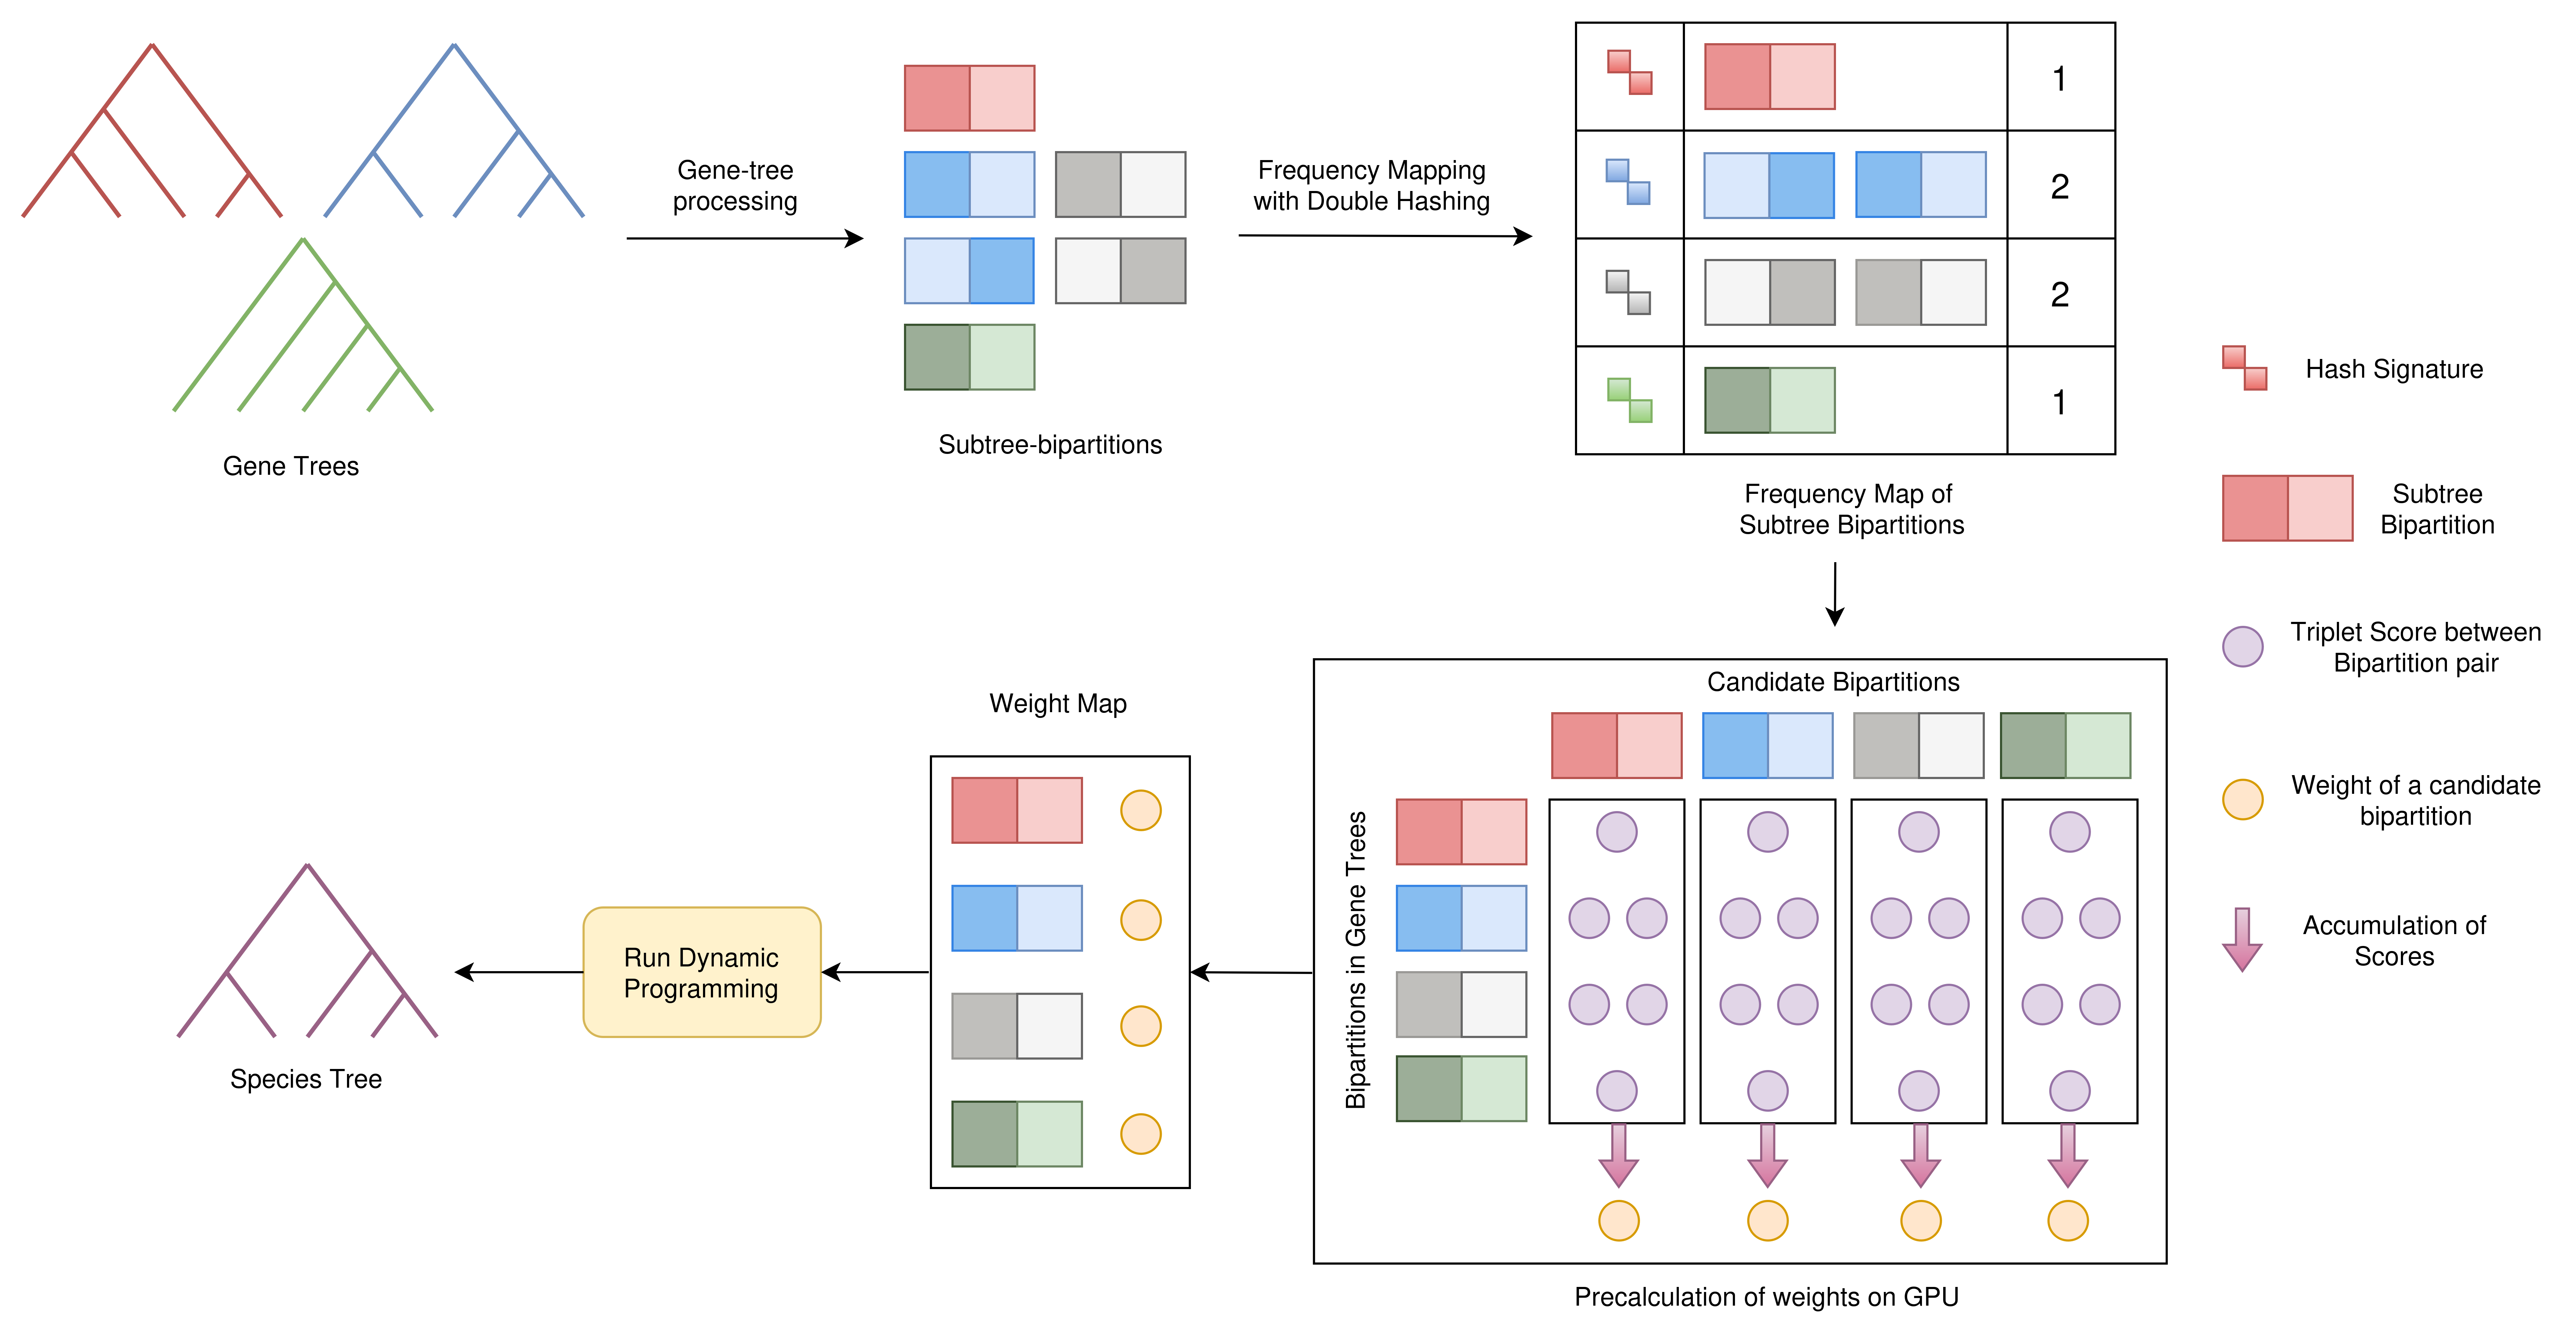
\includegraphics[width=0.9\linewidth]{fig-stx/v3-flow.png}
    \caption{Algorithmic framework of STELAR-X. First, the frequencies of unique subtree bipartitions across gene trees are determined using double hashing. Subsequently, the triplet consistency weights of all candidate bipartitions are precomputed in parallel on the GPU. The resulting weight map is then utilized within the dynamic programming to infer the species tree.}
    \label{fig:stelar-flow}
\end{figure}

% \subsection{Formation of Candidate Subtree-Bipartitions \addr{we do not need this here}}

% \textcolor{blue}{TODO: need to write the inclusion of consensus trees and cite ASTRAL here, explaining why we may need extra bipartitions, and also saying in limitation and future work that consensus tree finding might itself present a bottleneck so finding wayaround for that...} 

\subsection{Compact tuple representation of subtree bipartitions}
\label{subsec:tuple-representation}

For each gene tree $g_i$ we form an array $A_i$ of its leaf labels in a postorder traversal. Any internal node in $g_i$ induces a bipartition $(A|B)$ where $A$ and $B$, by construction, correspond to two adjacent contiguous subarrays of $A_i$. Let $\mathcal{A}_{i,l,r}$ denote the subarray of $\mathcal{A}_i$ from indices $l$ to $r$ (i.e., $A_{i}[l_1:r_1]$). Then, if $A = \mathcal{A}_{i,l_1,r_1}$ and $B = \mathcal{A}_{i,l_2,r_2}$, the bipartition $(A|B)$ can be represented as the tuple $(i,l_1,r_1,l_2,r_2)$, where $l_1 < r_1< l_2<r_2$. In fact, since $l_2 = r_1 + 1$, four integers suffice to store the bipartition. 

This tuple representation reduces storage from $O(n)$ bits per bipartition to a constant number of machine words, giving an overall space of $O(|\mathcal{CB}|)$ words. Because $|\mathcal{B}|=O(nk)$, the storage for the unique bipartitions is $O(nk)$ words, while the usual bitset representations would take  $O(n^{2}k)$ space.

\subsection{Frequency mapping of subtree-bipartitions using permutation-invariant and associative double hashing}
\label{subsec:freq-mapping}

We now describe the efficient construction of the frequency map $f_{\mathcal{G}}(x)$ of a subtree-bipartition $x in \mathcal{GB}$ across all gene trees in $\mathcal{G}$ under the compact integer-tuple representation. 

\paragraph{Equivalence of bipartitions.}
Let $P$ and $Q$ be sets of taxa; we write $P \sim Q$ if they contain the same taxa, regardless of order. Two subtree-bipartitions $x = (A_1 \mid B_1)$ and $y = (A_2 \mid B_2)$ are equivalent ($x \equiv y$) if either $A_1 \sim A_2$ and $B_1 \sim B_2$, or $A_1 \sim B_2$ and $B_1 \sim A_2$. Thus, equivalence is invariant under both taxon ordering and side swapping.

For bipartitions $x = (i_x,l_{1x},r_{1x},l_{2x},r_{2x})$ and $y = (i_y,l_{1y},r_{1y},l_{2y},r_{2y})$, equivalence is possible only when $i_x \neq i_y$ (i.e., two bipartitions originate from different gene trees). Bipartitions within the same gene tree ($i_x = i_y$) are either disjoint or one contains the other. A naive cross-tree comparison would require $O(n)$ time per pair. To eliminate this overhead, we adopt a hashing-based approach that detects equivalence in $O(1)$ time.


%Let $x = (i_x,l_{1x},r_{1x},l_{2x},r_{2x})$ and $y = (i_y,l_{1y},r_{1y},l_{2y},r_{2y})$ be two bipartitions. We distinguish two cases:
%\begin{description}
    %\item[Case 1: $i_x = i_y$.] Since both bipartitions arise from the same gene tree, their index ranges must either coincide exactly or be disjoint. In fact, two distinct bipartitions of the same tree cannot be equivalent. Therefore, $x \not\equiv y$.
    
   % \item[Case 2: $i_x \neq i_y$.] When bipartitions originate from different gene trees, equivalence is possible. A naïve approach would compare the sets of taxa directly, requiring $O(n)$ time. To avoid this overhead, we employ a hashing-based technique that is both efficient and reliable.
%\end{description}

\paragraph{Permutation-invariant double hashing.}
\label{para:hashing-and-freq-mapping}
We introduce a permutation-invariant and associative hash function $\phi$ that maps a set of taxa to a single hash value independent of order. Associativity enables the use of prefix-scan arrays for constant-time subarray hashing \addr{did not understand it. talk to Anik}. If $x \equiv y$, then by definition,
\[
\phi(A_{1x}) = \phi(A_{1y}) \ \text{and}\  \phi(B_{1x}) = \phi(B_{1y}), 
\]
or the corresponding equalities under a side swap. Although equal hash values suggest possible equivalence, hash collisions prevent a strict guarantee. To make the probability of collisions negligible, we employ two safeguards.


 First, we apply double hashing: two independent permutation-invariant and associative hash functions, $\phi_1$ and $\phi_2$, produce a composite signature $(\phi_1, \phi_2)$ for each bipartition.
Second, we apply a per-element hash function $\mathcal{H}$ to each taxon identifier $d_j \in \{0,\ldots,n-1\}$, projecting it into a large finite field $\mathbb{F}_P$ via multiplication and bitwise operations modulo a large prime $P$. \addr{did I write it correct?}\textcolor{blue}{Sir, the implementation actually uses a bit more convoluted function in this place. I have written as such...}. This sparse projection decorrelates nearby identifiers and prevents structural collisions common to contiguous integer labels \addr{this is a compact version of the following. is it okay?}\textcolor{blue}{Yes, Sir}. Thus, for a subset $S$ of taxa, we define its set-level signature as $\sigma(S) = (\phi_1({r_j : j \in S}),, \phi_2({r_j : j \in S}))$, where each $r_j = \mathcal{H}(d_j) \in \mathbb{F}_P$. Consequently, for a bipartition $x = (A|B)$, the composite signature becomes $(\sigma(A), \sigma(B))$.
% This projection is essential because permutation-invariant hash functions such as SUM or XOR, when applied directly to small, contiguous identifiers, exhibit higher collision probabilities due to their limited combinatorial diversity. By first dispersing identifiers through $\mathcal{H}$, we ensure that the resulting hash space is sparse and the likelihood of accidental collisions is negligible.


For each subarray $\mathcal{A}_{i,l,r}$, we compute
\[
\phi_1(\{\mathcal{H}(d_j)\}_{l \le j \le r}), \quad
\phi_2(\{\mathcal{H}(d_j)\}_{l \le j \le r}).
\]

Leveraging associativity, we precompute prefix-scan arrays for $\phi_1$ and $\phi_2$, enabling $O(1)$ computation of subarray hash values. All arithmetic is performed modulo a large prime $P$ (e.g., $2^{61}-1$). Finally, the frequency $f_\mathcal{G}(x)$ of each unique bipartition $x \in \mathcal{GB}$ is derived by inserting the computed signatures into a hash table and counting the number of equivalent bipartitions that share the same hash value.
Figure~\ref{fig:double-hashing} illustrates this process.

The combination of double hashing and sparse integer mapping makes collisions vanishingly rare (see the collision analysis in Theorem~\ref{thm:collision-probability}). In our implementation, $\phi_1$ is SUM and $\phi_2$ is XOR over $\mathbb{F}_P$, and we observed no hash collisions even on datasets with 100K taxa and 100K genes. 

\begin{figure}
    \centering
    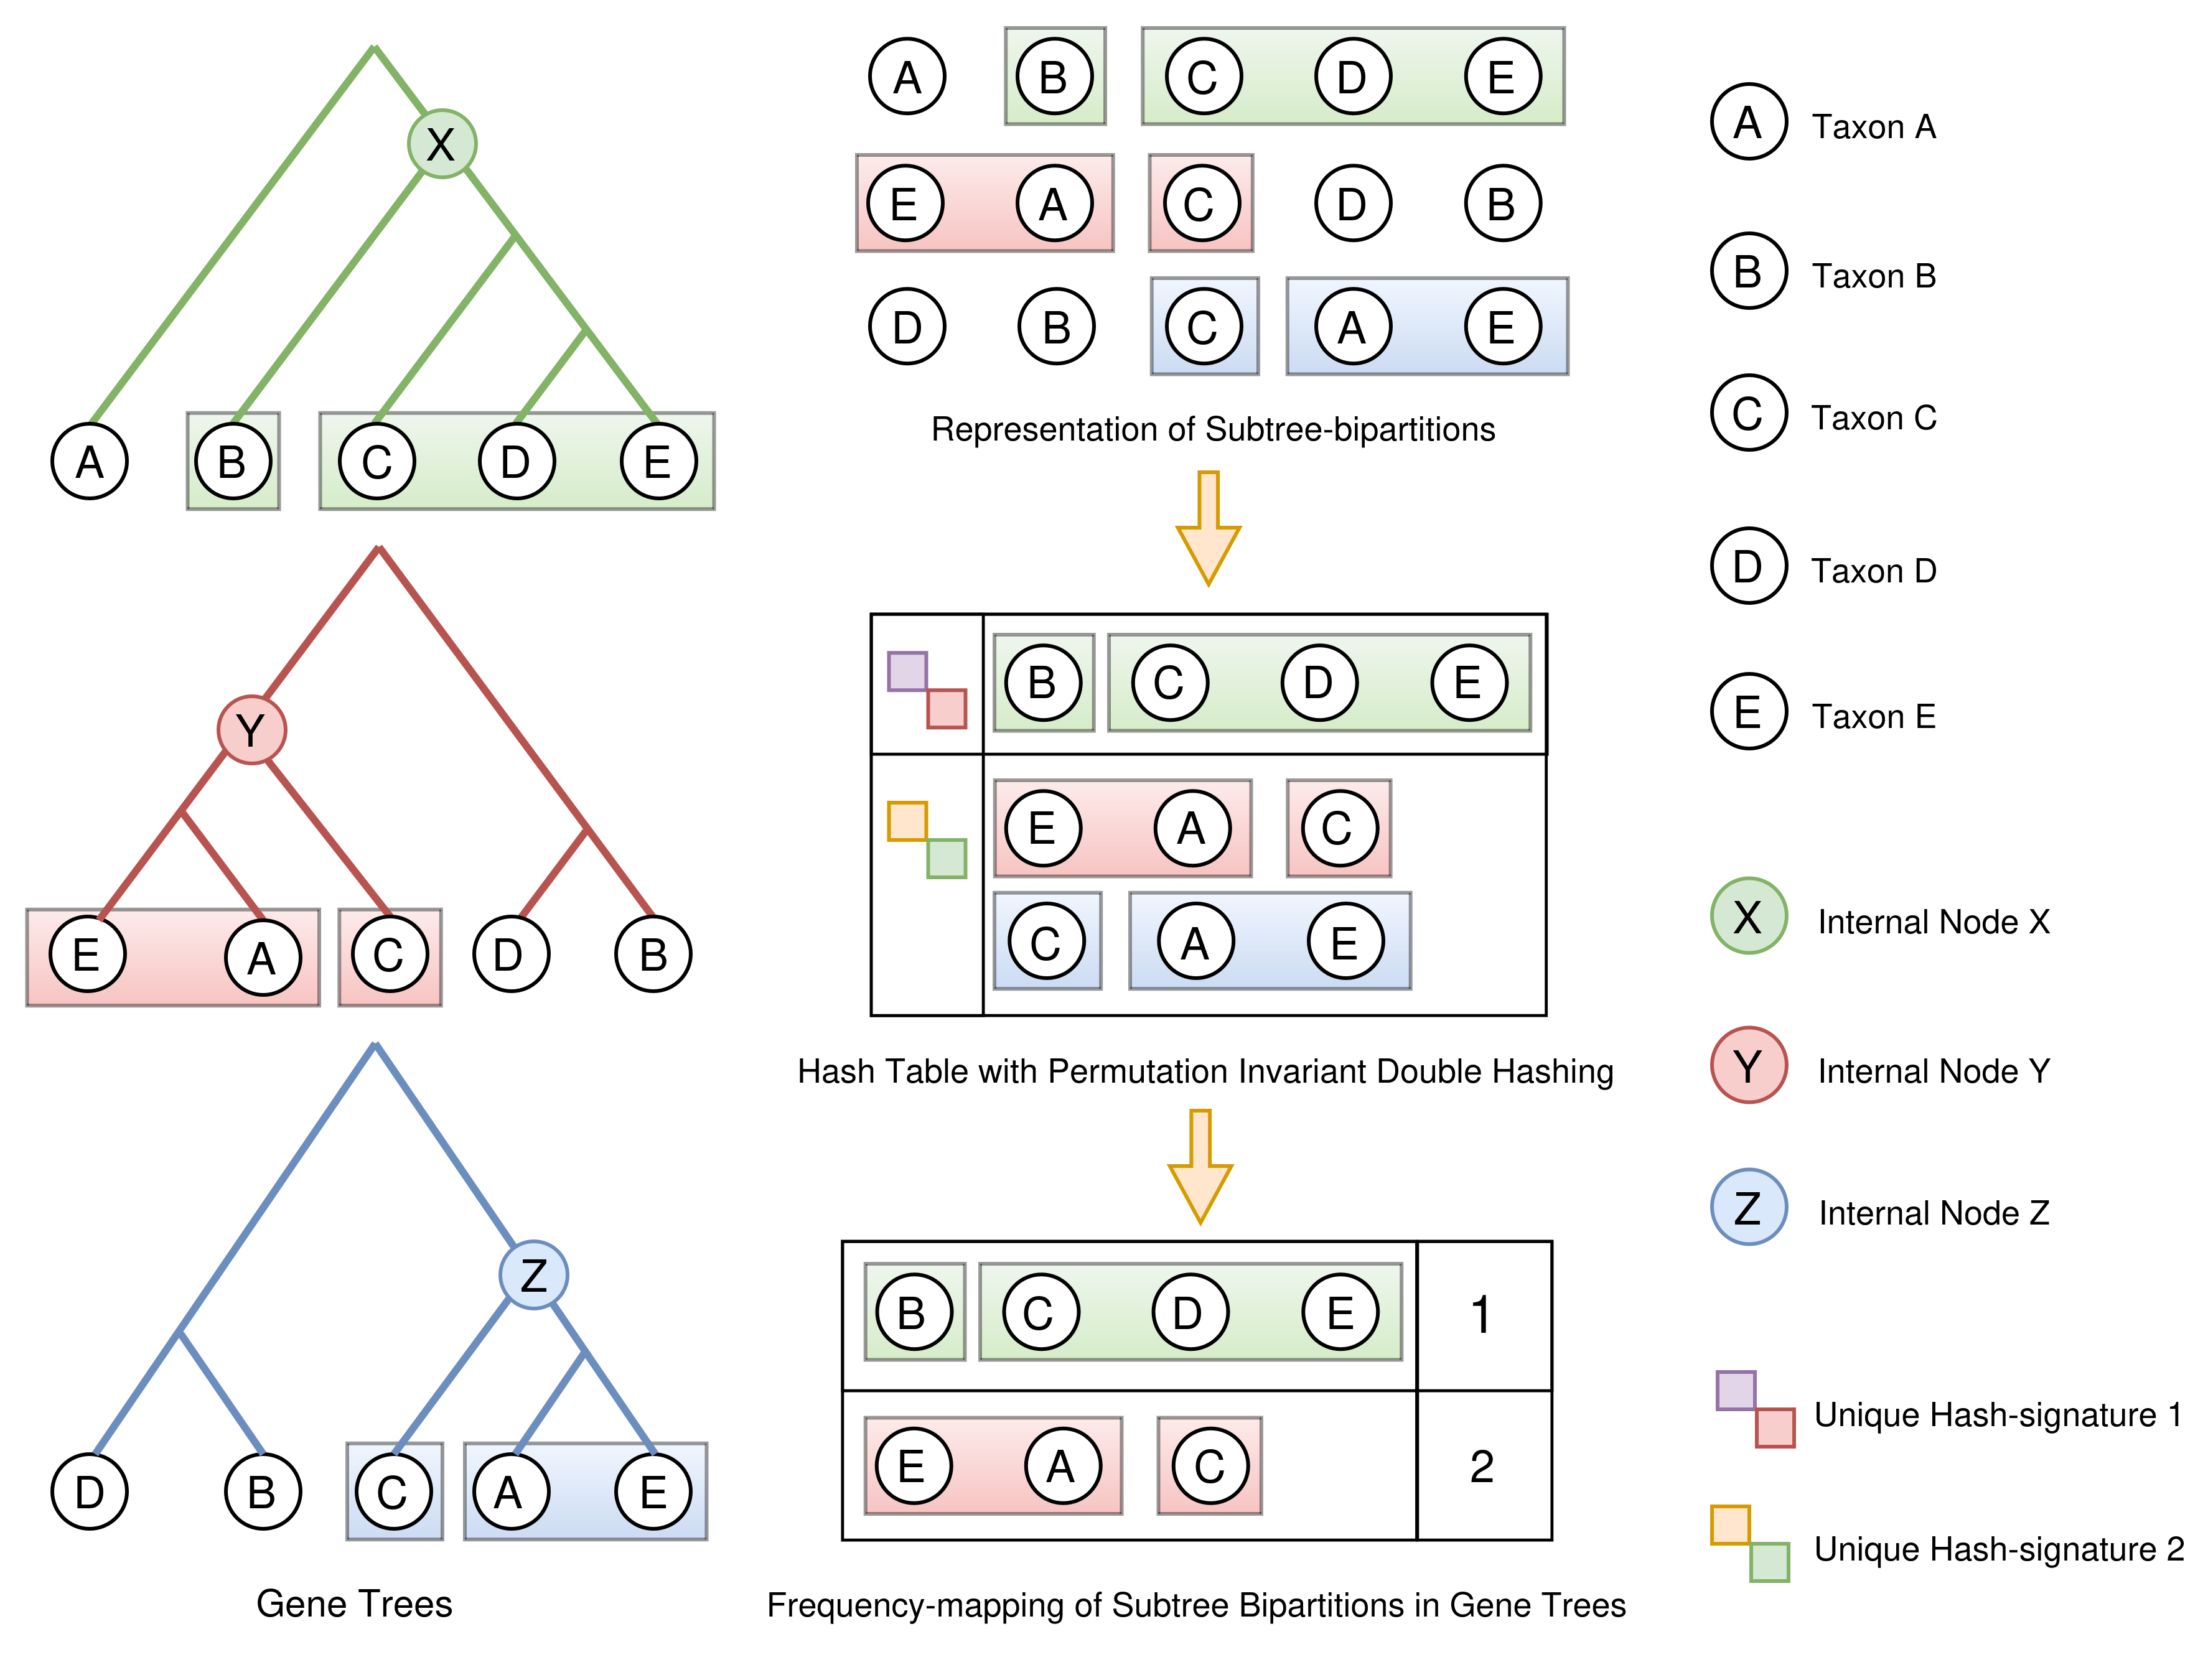
\includegraphics[width=0.75\linewidth]{fig-stx/v5-freq.png}
    \caption{Example scenario of the frequency mapping of subtree-bipartitions with permutation-invariant double hashing. Three example subtree-bipartitions $(B|CDE)$, $(EA|C)$, and $(C|AE)$ are considered from the input gene trees. Since $(EA|C)$ and $(C|AE)$ are equivalent, they are mapped to the same hash-signature, enabling the subsequent determination of its frequency as 2.}
    \label{fig:double-hashing}
\end{figure}

\begin{theorem}[Collision Probability Bound]
\label{thm:collision-probability}
Let $\sigma(S) = (\phi_1(\{r_j : j \in S\}),\, \phi_2(\{r_j : j \in S\}))$ be the double-hash signature of a taxon subset $S$, where $\phi_1,\phi_2$ are independent permutation-invariant hash functions over $\mathbb{F}_P$ and each $r_j = \mathcal{H}(d_j)$ is independently and uniformly distributed in $\mathbb{F}_P$.  
Among $M$ total bipartitions, the probability that at least one collision will occur is bounded by
\[
\Pr(\exists\ \text{collision}) \le \frac{M^2}{P^2}.
\]
\end{theorem}

\noindent
\textit{Proof.} See Supplementary Material~A.

Thus, to keep this probability below a prescribed tolerance $\delta$, it suffices to ensure that
\(
P \;\geq\; \frac{M}{\sqrt{\delta}}.
\).
Hence, choosing $P$ sufficiently larger than $M$ renders global collisions negligible in practice.


\paragraph{Theoretical Analysis of Collision Probability}  

Now we provide a theoretical analysis of the probability of collisions. The key intuition is that collisions are rare because whenever two sets differ, at least one taxon contributes an independent random value, making accidental equality highly unlikely.

Let $\mathcal{X}$ be the taxon set with $|\mathcal{X}|=n$. Let $M$ be the number of subtree-bipartitions produced across all gene trees (in our setting, $M=\Theta(nk)$). We choose a large prime $P$ and work in the field $\mathbb{F}_P$.

\textbf{Setup.} A single-element hash
\[
\mathcal{H}:\{0,\dots,n-1\}\to\mathbb{F}_P
\]
maps each taxon identifier $d_j$ to
\[
r_j \coloneqq \mathcal{H}(d_j)\in\mathbb{F}_P.
\]
We idealize that the values $\{r_j\}_{j=1}^n$ are independent and uniformly distributed in $\mathbb{F}_P$.

We then apply two associative, permutation-invariant set-level functions $\phi_1,\phi_2$, each operating directly on subsets of $\{r_j\}$. The signature of a set $S$ is
\[
\sigma(S) \coloneqq \big(\phi_1(\{r_j:j\in S\}),\, \phi_2(\{r_j:j\in S\})\big).
\]

\textbf{Single-set collision probability.}  
Let $S\neq T$ and define $U=S\setminus T$, $V=T\setminus S$. Associativity ensures that $\phi_a$ admits a natural cancellation operator $\ominus$ (e.g. subtraction for addition, XOR for XOR, etc.), so that
\[
\phi_a(S)\ominus\phi_a(T) \;=\; \phi_a(U)\ominus\phi_a(V).
\]
Because $U\cup V\neq\varnothing$, at least one $r_t$ appears only in one side. Conditioning on all other $r_j$, the difference reduces to a function of the uniform random variable $r_t$. This equals zero with probability at most $1/P$. Thus
\begin{equation}\label{eq:single-hash}
\Pr\big(\phi_a(S)=\phi_a(T)\big) = \frac{1}{P}.
\end{equation}

\textbf{Pairwise signature collision.}  
Suppose the two set-level functions $\phi_1$ and $\phi_2$ are constructed so that their collision events are statistically independent (e.g.\ by using independent salts or structurally distinct definitions of $\phi_a$). Then for distinct sets $S,T$,
\[
\Pr\big(\sigma(S)=\sigma(T)\big)
= \Pr\big(\phi_1(S)=\phi_1(T)\big)\cdot \Pr\big(\phi_2(S)=\phi_2(T)\big)
= \frac{1}{P^2}.
\]



\textbf{Collision probability for bipartitions.}  
Let bipartitions $x=(A_1 \mid B_1)$ and $y=(A_2 \mid B_2)$ be distinct (non-equivalent).  
A collision occurs if and only if
\[
\big(\sigma(A_1)=\sigma(A_2)\ \wedge\ \sigma(B_1)=\sigma(B_2)\big)
\quad\text{or}\quad
\big(\sigma(A_1)=\sigma(B_2)\ \wedge\ \sigma(B_1)=\sigma(A_2)\big).
\]
Since each matching holds with probability $1/P^2$, we obtain
\[
\Pr\!\big(\text{collision between }x\text{ and }y\big) \;\le\; \frac{2}{P^2}.
\]




\textbf{Global (any-pair) collision probability.}  
Among $M$ bipartitions there are at most $\binom{M}{2}$ pairs. By a union bound,
\[
\Pr(\exists\ \text{collision}) \;\le\; \binom{M}{2}\cdot \frac{2}{P^2}
\;\le\; \frac{M^2}{P^2}.
\]






\subsection{Precomputation of Bipartition Weights}
\label{subsec:weight-precomp}

We next justify and describe the precomputation of weights associated with all candidate bipartitions in $\mathcal{CB}$. This step is essential for the dynamic programming (DP) phase of STELAR, whose state space is defined by the recursive formulation in Equation~\eqref{eq:recurrence-relation}. % As illustrated in Figure~\ref{fig:stelar-dp} \addr{remove this part if we omit the figure}, 
The DP begins with the full taxon set $\mathcal{X}$ and recursively partitions each cluster using subtree-bipartitions. Consequently, every transition depends on the availability of bipartition weights.  We now show that, in the constrained version of STELAR, this process inevitably requires the weights of all subtree-bipartitions in $\mathcal{GB}$.

\begin{theorem}
\label{th:dp-span}
If $\mathcal{CB} = \mathcal{GB}$, then the DP state space spans every subtree-bipartition $x \in \mathcal{CB}$.
\end{theorem}

\begin{proof}
    \addb{See Appendix X}
    We argue by contradiction. Suppose there exists a bipartition $x = (A|B) \in \mathcal{CB}$ that is not explored in the state space of the DP. We consider two possible cases:

    \begin{description}
        \item[Case 1: $A \cup B = \mathcal{X}$]  
        Since $\mathcal{CB} = \mathcal{GB}$, we have $x \in \mathcal{GB}$. As $A \cup B$ covers all taxa, $x$ corresponds to a root-level bipartition in one of the gene trees. By construction, such bipartitions are included in the search space at the very first state transition. This contradicts our assumption that $x$ is not explored.

        \item[Case 2: $A \cup B \neq \mathcal{X}$]  
        Again, $x \in \mathcal{GB}$ and hence arises from some internal node $u$ of a gene tree $g_i$, where the taxa covered by $u$ form the set $\mathcal{Y} = A \cup B$. Since $\mathcal{Y} \subsetneq \mathcal{X}$, $u$ must have a parent node $p$ in $g_i$. Let the bipartition induced by $p$ be $y = (C|D)$. By construction, either $C = \mathcal{Y}$ or $D = \mathcal{Y}$. Thus, if $y$ is explored in the DP state space, then the algorithm must also explore its child bipartition $x$, by design of the transition rules. Hence, the assumption that $x$ is not explored implies that $y$ is also not explored. Repeating this reasoning along the ancestor chain of $u$, we eventually reach the root of $g_i$, where Case~1 applies and yields a contradiction.
    \end{description}

    Since both cases lead to contradictions, our assumption is false. Therefore, every subtree-bipartition $x \in \mathcal{GB}$ is necessarily explored in the constrained DP state space. Thus, precomputing weights is reasonable and justifies isolating this step for GPU acceleration.
\end{proof}

Even when $\mathcal{GB} \subsetneq \mathcal{CB}$, precomputing weights for all $x \in \mathcal{CB}$ remains practical as long as $|\mathcal{CB}|$ is not asymptotically larger than $|\mathcal{GB}|$.

%This result shows that, in the constrained setting where $\mathcal{CB} = \mathcal{GB}$, the dynamic programming algorithm must access the weights of all bipartitions in $\mathcal{GB}$. Furthermore, even when $\mathcal{GB} \subsetneq \mathcal{CB}$, as long as $|\mathcal{CB}|$ is not asymptotically larger than $|\mathcal{GB}|$, it remains practical to precompute the weights of all subtree-bipartitions in $\mathcal{CB}$.


\paragraph{Weight formulation.}
Let $x = (A_1 \mid B_1) \in \mathcal{CB}$ be a candidate bipartition and $y = (A_2 \mid B_2) \in \mathcal{SBP}(g_i)$ a bipartition from gene tree $g_i$.  
Following~\cite{stelar}, the number of triplets simultaneously mapped to both $x$ and $y$ is
\begin{equation}
\mathcal{M}(x,y) = 
\mathcal{NT}(|A_1 \cap A_2|, |B_1 \cap B_2|) +
\mathcal{NT}(|A_1 \cap B_2|, |A_2 \cap B_1|),
\label{eq:Mxy}
\end{equation}
where $\mathcal{NT}(n_1,n_2)$ is the number of triplets mapped to a bipartition $(A \mid B)$ with $|A| = n_1$, $|B| = n_2$:
\begin{equation}
\mathcal{NT}(n_1,n_2) = 
\binom{n_1}{2}\binom{n_2}{1} + 
\binom{n_2}{2}\binom{n_1}{1}
= \frac{n_1 n_2 (n_1 + n_2 - 2)}{2}.
\label{eq:NT}
\end{equation}
The total weight of $x$ across all gene trees is then
\begin{equation}
w_{\mathcal{G}}(x) = \sum_{i=1}^{k} \ \sum_{y \in \mathcal{SBP}(g_i)} \mathcal{M}(x,y).
\end{equation}

Using the precomputed frequency mapping $f_{\mathcal{G}}(y)$ of unique bipartitions $y \in \mathcal{GB}$ produced by the double hash table, this can be written more efficiently as
\begin{equation}
w_{\mathcal{G}}(x) = \sum_{y \in \mathcal{GB}} f_{\mathcal{G}}(y) \, \mathcal{M}(x,y).
\label{eq:effcal}
\end{equation}

Note that each $M(x,y)$ requires computing the four intersection cardinalities  between clusters $|A_1\cap A_2|,|B_1\cap B_2|,|A_1\cap B_2|,|A2\cap B_1|$ (Equations~\eqref{eq:Mxy} and \eqref{eq:NT}).

\paragraph{Efficient intersection counting using tuples.} 
To avoid memory-intensive bitset operations, we employ our proposed integer-tuple representation of subtree-bipartitions.  
Let $X = \mathcal{A}_{i,l_x,r_x}$ and $Y = \mathcal{A}_{j,l_y,r_y}$ denote two clusters ($i \neq j$).  
We have $|X| = r_x - l_x + 1$ and $|Y| = r_y - l_y + 1$.  
The intersection $|X \cap Y|$ is computed by iterating over each taxon in the smaller cluster and checking taxon membership in the other cluster.  To optimize this membership testing, we precompute index maps $\pi_i(v)$, where $\pi_i(v)$ gives the position of taxon $v$ in the post order array representation $\mathcal{A}_i$ of $g_i$. Thus, for each taxon $v \in \mathcal{A}_{i,l_{x},r_{x}}$, we check whether $l_y \leq \pi_j(v) \leq r_y$ and accumulate the intersection count. This procedure runs in $O(\min(|X|, |Y|))$ time per intersection.

\[
|X \cap Y| = 
\sum_{v \in \mathcal{A}_{i,l_x,r_x}} 
\mathbf{1}_{[\,l_y \le \pi_j(v) \le r_y\,]}.
\]


%We now present a theoretical bound on the running time of this precomputation over all the bipartitions under balanced gene-tree assumption. 
Assuming balanced gene trees, the total time for precomputing all $w_{\mathcal{G}}(x)$ over $\mathcal{GB}$ is $O(n^2 k^2)$ (Theorem~\ref{th:precompute-bound}).  
This justifies isolating the weight precomputation as a separate stage, which we further accelerate using GPU parallelization (see Section~\ref{subsec:parallel}). Although the analysis assumes perfectly balanced binary trees for mathematical convenience, the practical runtime depends mainly on the smaller of the two subtrees in each bipartition pair and thus, the observed running time remains close to the theoretical bound under typical conditions. Noticeable deviations occur only when most gene trees are highly unbalanced, but this effect is mitigated in practice since the number of unique bipartitions $|\mathcal{GB}|$ is usually much smaller than $nk$. Thus, the balanced-tree assumption offers a good approximation of real-world performance.




\begin{theorem}
\label{th:precompute-bound}
Assume $\mathcal{CB} = \mathcal{GB}$, where $\mathcal{GB}$ contains all subtree bipartitions across the $k$ gene trees. In other words, every bipartition across all gene trees is unique. If each gene tree is a perfectly balanced rooted binary tree with $n = 2^{d}$ taxa, then the precomputation of weights requires $\mathcal{O}(n^{2}k^{2})$ time.

\end{theorem}

\begin{proof}
\addr{Proof is provided in Appendix Y}. By Equation~\eqref{eq:effcal}, computing the weight of each candidate
bipartition requires evaluating \(\mathcal{M}(x,y)\) against every
\(y\in\mathcal{GB}\). Thus we must evaluate \(\mathcal{M}(x,y)\) for
every ordered pair \((x,y)\in\mathcal{GB}\times\mathcal{GB}\). We bound
the total cost by first bounding the cost between two fixed balanced
trees and then summing over the tree-pairs.

In a perfectly balanced rooted binary tree on \(n=2^{d}\) leaves,
an internal node at depth \(\ell\) (root at depth \(0\)) has subtree
size \(n/2^{\ell}\), and each of its two child subtrees has size
\(s = n/2^{\ell+1}\). Thus the set of possible child-subtree sizes is
\[
\mathcal{S}=\{\,2^{0},2^{1},\dots,2^{d-1}\,\},
\]
and for a given child-subtree size \(s\in\mathcal{S}\) the number of
internal nodes whose child-subtrees have size \(s\) equals the number of
disjoint blocks of size \(2s\) that partition the \(n\) leaves, i.e.
\(\frac{n}{2s}\). Therefore the number of subtree-bipartitions in one balanced tree whose parts (child-subtrees) have size \(s\)
is \(n/(2s)\).

\textbf{Per-pair cost in terms of sizes.}
We consider two bipartitions \(x=(A_{1}|B_{1})\) in tree \(g_p\) and
\(y=(A_{2}|B_{2})\) in tree \(g_q\), and let the child-subtree sizes
be \(s\) and \(t\), respectively. So \(|A_{1}|=|B_{1}|=s\) and
\(|A_{2}|=|B_{2}|=t\)). By Equation~\eqref{eq:Mxy}, \(\mathcal{M}(x,y)\)
depends on four intersection counts among the parts of \(x\) and
\(y\). Each such intersection can be computed by iterating over the
smaller argument using the index map \(\pi\), hence the time to compute each intersection is \(O(\min(s,t))\). Since there are only a constant number of
such intersections, the total cost to evaluate \(\mathcal{M}(x,y)\) is
\[
\operatorname{cost}(\mathcal{M}(x,y)) \;=\; O(\min(s,t)).
\]

\textbf{Cost between two balanced trees.}
We now group bipartitions of \(g_p\) and \(g_q\) by their child-subtree sizes
\(s=2^{i}\) and \(t=2^{j}\) (with \(0\le i,j\le d-1\)). The number of
bipartitions in \(g_p\) with part-size \(s\) is \(n/(2s)\), and similarly
for \(g_q\) with part-size \(t\). Thus the number of ordered bipartition
pairs with sizes \((s,t)\) is \(\frac{n}{2s}\cdot\frac{n}{2t}\), and the
contribution of this size-class pair to the cost is
\[
\frac{n}{2s}\cdot\frac{n}{2t}\cdot O(\min(s,t))
= O\!\left(\frac{n^{2}\min(s,t)}{4st}\right)
= O\!\left(\frac{n^{2}}{4\max(s,t)}\right).
\]
Replacing \(s=2^{i}\) and \(t=2^{j}\), the total cost between the two
trees is
\[
S_{pq} \;=\; O\!\left(n^{2}\sum_{i=0}^{d-1}\sum_{j=0}^{d-1} 2^{-\max(i,j)}\right).
\]


We evaluate the double sum by symmetry. Splitting the domain into the two
triangles \(i\le j\) and \(i>j\):
\begin{align*}
\sum_{i=0}^{d-1}\sum_{j=0}^{d-1}2^{-\max(i,j)}
&=\sum_{j=0}^{d-1}\sum_{i=0}^{j}2^{-j}
  +\sum_{i=0}^{d-1}\sum_{j=0}^{i-1}2^{-i} \\[4pt]
&=\sum_{j=0}^{d-1}(j+1)2^{-j}
  +\sum_{i=0}^{d-1}i\,2^{-i} \\[4pt]
&=2\sum_{k=0}^{d-1}\frac{k}{2^{k}}
  +\sum_{k=0}^{d-1}\frac{1}{2^{k}}.
\end{align*}
Both finite sums are uniformly bounded as \(d\) grows, since
\(\sum_{k\ge0}k/2^{k}=2\) and \(\sum_{k\ge0}1/2^{k}=2\).
Hence
\[
\sum_{i=0}^{d-1}\sum_{j=0}^{d-1}2^{-\max(i,j)} \le 6,
\]
and in fact the exact value is
\[
\sum_{i=0}^{d-1}\sum_{j=0}^{d-1}2^{-\max(i,j)}
=6-\frac{2d+3}{2^{\,d-1}}.
\]
Therefore the double sum is \(O(1)\).




Hence \(S_{pq}=O(n^{2})\). Thus, computing all pairwise
intersection costs between bipartitions of two balanced trees costs
\(O(n^{2})\).

\textbf{Extension to $k$ trees.}
There are \(k\) gene trees and thus \(k^{2}\) ordered pairs of trees.
Summing the \(O(n^{2})\) cost over all ordered pairs yields the
total precomputation cost
\(O(n^{2})\cdot k^{2}=O(n^{2}k^{2})\), which proves the theorem.
\end{proof}

Our analysis assumes perfectly balanced binary trees for mathematical tractability. However, because the runtime for each bipartition pair primarily depends on the minimum of the corresponding subtree sizes, the overall running time is expected to remain close to the derived asymptotic bound in realistic scenarios. Only in extreme cases where most gene trees are highly unbalanced would we incur notable deviations. In practice, such imbalance is further mitigated by the fact that the number of unique bipartitions, $|\mathcal{GB}|$, is generally smaller than $nk$. Hence, the balanced-tree assumption provides a reasonable approximation of empirical behavior.





\textcolor{blue}{Sir, here I have added the proof for the caterpillar case, It turns out to be $O(n^3k^2)$.}

\begin{theorem}
\label{th:caterpillar-worst}
Assume $\mathcal{CB}=\mathcal{GB}$ and that $\mathcal{GB}$ contains all subtree bipartitions across the $k$ gene trees. If each gene tree is a rooted caterpillar on $n$ taxa, then the precomputation of weights (evaluating $\mathcal{M}(x,y)$ for all ordered pairs $x,y\in\mathcal{GB}$) requires $\mathcal{O}(n^{3}k^{2})$ time.
\end{theorem}

\begin{proof}
By Equation~\eqref{eq:effcal}, the precomputation requires computing
\(\mathcal{M}(x,y)\) for every ordered pair \((x,y)\in\mathcal{GB}\times\mathcal{GB}\).
We first bound the cost between two fixed caterpillar trees and then sum
over all ordered tree pairs.

\medskip\noindent\textbf{Bipartitions in a rooted caterpillar.}
Fix a rooted caterpillar on \(n\) leaves arranged along the backbone.
Its internal nodes (listed from the root downwards) induce the bipartitions
\[
(1 \mid n-1),\; (1 \mid n-2),\; \dots,\; (1 \mid 1),
\]
where each ordered pair denotes a leaf set on the left and its complement
on the right. Equivalently, for each \(L\in\{1,\dots,n-1\}\) there is
exactly one bipartition whose large side has size \(L\) (and the
small side is size \(1\)). Thus each caterpillar has exactly \(n-1\)
subtree-bipartitions and the multiset of large-side sizes is
\(\{1,2,\dots,n-1\}\) (each appearing once).

\medskip\noindent\textbf{Per-pair computation of \(\mathcal{M}(x,y)\).}
For two bipartitions
\(x=(A_1\mid B_1)\) and \(y=(A_2\mid B_2)\) the equation
\eqref{eq:Mxy} requires four intersection counts:
\(|A_1\cap A_2|,\ |A_1\cap B_2|,\ |B_1\cap A_2|,\ |B_1\cap B_2|\).
In a rooted caterpillar at least three of these intersections involve a
singleton side (size \(1\)) and are therefore computable in \(O(1)\) time. The remaining intersection is the
one between the two large sides (say sizes \(s\) and \(t\)); this
intersection can be computed in \(O(\min(s,t))\) time by iterating over
the smaller large-side and checking membership via the index map. Thus
the dominant cost for evaluating \(\mathcal{M}(x,y)\) is
\[
\operatorname{cost}\big(\mathcal{M}(x,y)\big) \;=\; O\!\big(\min(s,t)\big),
\]
where \(s\) and \(t\) are the sizes of the large sides of \(x\) and \(y\),
respectively.

\medskip\noindent\textbf{Cost between two caterpillar trees.}
Each of the two caterpillar trees has exactly one bipartition whose
large-side size equals \(L\) for each \(L\in\{1,\dots,n-1\}\). Hence the
total cost between two trees equals
\[
S_{pq} \;=\; \sum_{s=1}^{n-1}\sum_{t=1}^{n-1} O\!\big(\min(s,t)\big)
\;=\; O\!\left(\sum_{s=1}^{n-1}\sum_{t=1}^{n-1}\min(s,t)\right).
\]
The inner double sum is a standard combinatorial sum; counting by the
minimum value \(m=\min(s,t)\) gives
\[
\sum_{s=1}^{n-1}\sum_{t=1}^{n-1}\min(s,t)
= \sum_{m=1}^{n-1} m\cdot\#\{(s,t):\min(s,t)=m\}.
\]
For a fixed \(m\), the number of ordered pairs \((s,t)\) with
\(\min(s,t)=m\) equals \(2(n-1-m)+1 = 2n-2m-1\). Therefore
\begin{align*}
\sum_{s=1}^{n-1}\sum_{t=1}^{n-1}\min(s,t)
&= \sum_{m=1}^{n-1} m(2n-2m-1)
= 2n\sum_{m=1}^{n-1} m - 2\sum_{m=1}^{n-1} m^2 - \sum_{m=1}^{n-1} m \\
&= \Theta(n^3).
\end{align*}
(Using the closed forms \(\sum_{m=1}^{n-1} m = \Theta(n^2)\) and
\(\sum_{m=1}^{n-1} m^2 = \Theta(n^3)\) one obtains the cubic bound.)
Hence \(S_{pq} = O(n^3)\).

\medskip\noindent\textbf{Extension to \(k\) trees.}
There are \(k\) gene trees and thus \(k^{2}\) ordered tree-pairs. Summing
the per-pair bound \(O(n^{3})\) over all ordered pairs yields the total
precomputation cost
\[
O(n^{3})\cdot k^{2} = O(n^{3} k^{2}),
\]
which completes the proof.
\end{proof}













\subsection{Execution of Dynamic Programming}
\label{subsec:dp}

As the final stage, we execute the dynamic programming (DP) procedure defined by Equation~\eqref{eq:recurrence-relation}. Each DP state corresponds to a cluster of taxa, and transitions require identifying all subtree-bipartitions $x \in \mathcal{CB}$ that partition the taxa in the current cluster. To enable efficient lookup, we precompute a state-space mapping $\Psi$ from clusters $C\subseteq X$ hashes) to the set of candidate bipartitions. 
\[
\Psi : \{\text{clusters of taxa}\} \;\longrightarrow\; \mathcal{CB},
\qquad 
% \Phi(A \cup B) = \{\, x = (A|B) \,\}.
\Psi(C) = \{\, x = (A|B) \in \mathcal{CB} \mid A \cup B = C \,\}.
\]

For each subtree-bipartition $x = (A|B) \in \mathcal{CB}$, we define its associated cluster $C = A \cup B$ and construct a mapping. Here, again, we employ the double-hashing scheme as before and avoid the memory-intensive bitset representation. Each cluster $C$ is encoded using the pair of hash signatures $(\phi_1(C), \phi_2(C))$.

During DP (Eq.~\ref{eq:dp}) we enumerate $\Psi(C)$ to obtain allowed subtree-bipartitions and fetch $w_{\mathcal{G}}(A|B)$ in $O(1)$ time per bipartition using the precomputed weight map discussed earlier (Sec~\ref{subsec:weight-precomp}). Because both the state space (clusters) and candidate bipartitions are encoded via compact signatures, memory demand remains $O(|\mathcal{C}|+|\mathcal{B}|)=O(nk)$. The DP itself then runs in time proportional to the number of state transitions (i.e., the total number of candidate bipartitions considered), plus any bookkeeping overhead.
 % The overall workflow of this procedure is illustrated in Figure~\ref{fig:stelar-dp} \addb{this figure is not that necessary}.


% \begin{figure}
%     \centering
%     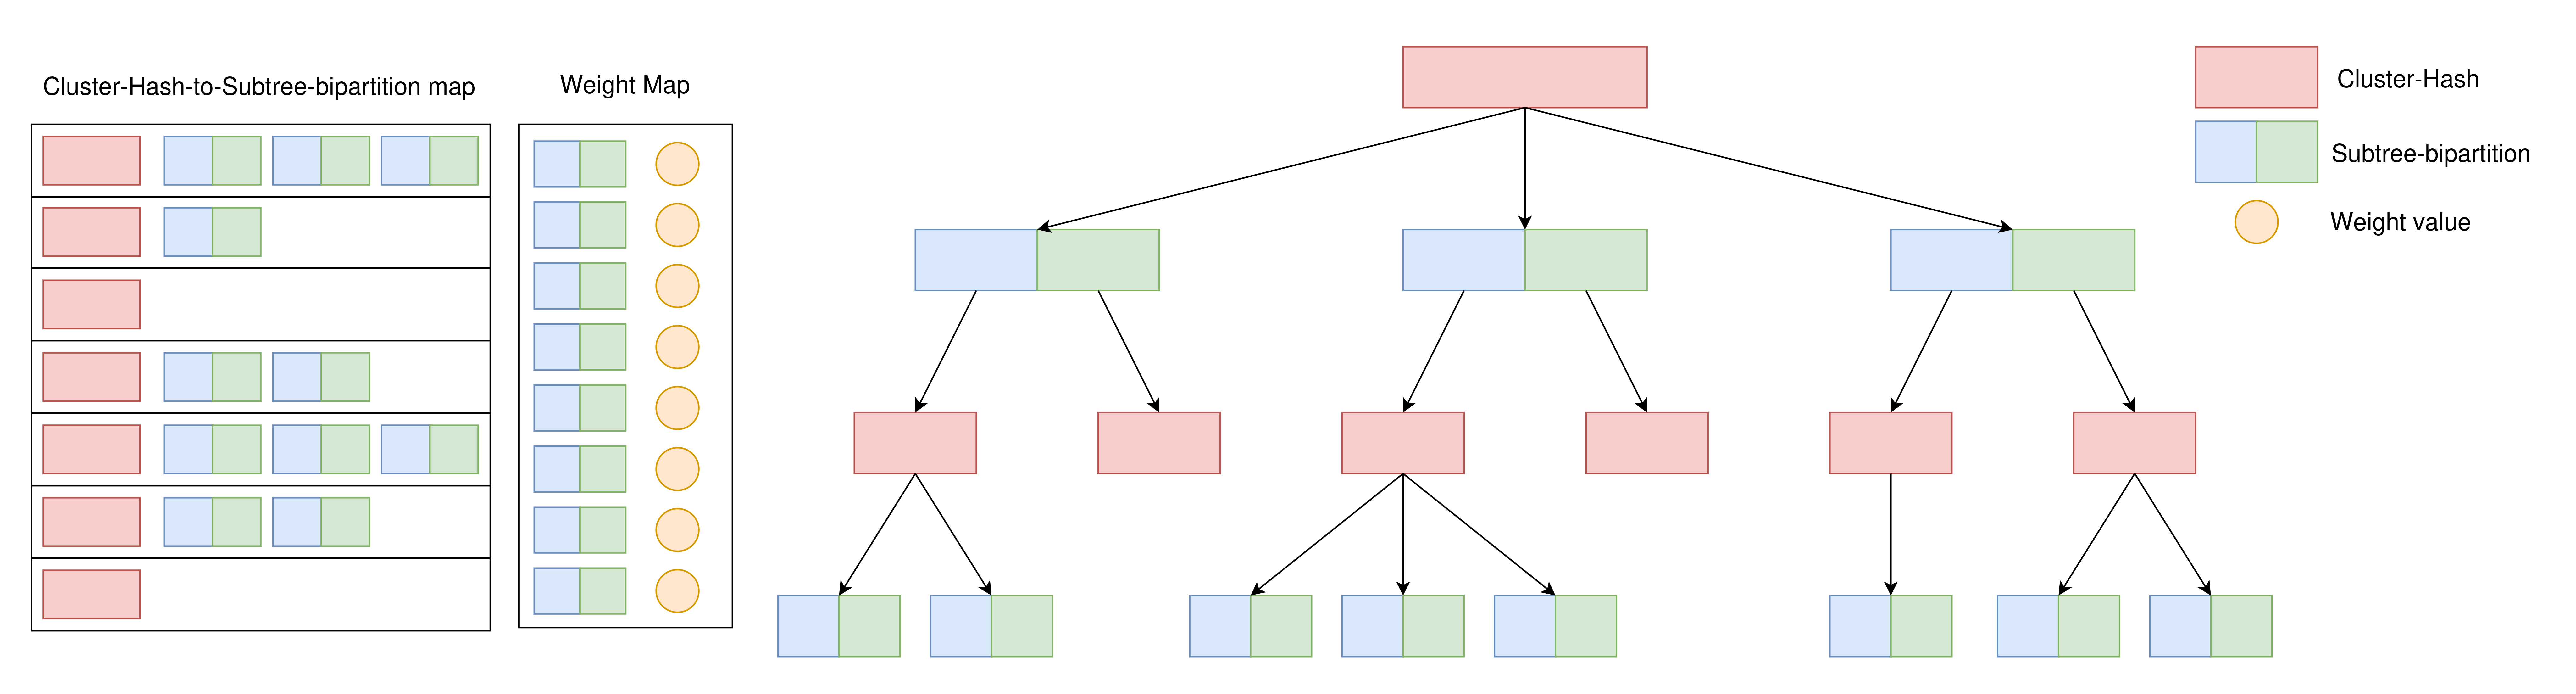
\includegraphics[width=0.98\linewidth]{fig-stx/v3-dp-alg.png}
%     \caption{Dynamic programming algorithm in STELAR-X using cluster-hash to subtree-bipartition map and precomputed weight map}
%     \label{fig:stelar-dp}
% \end{figure}

\subsection{Parallelization}
\label{subsec:parallel}


We next identify the stages of our algorithm that are amenable to CPU and GPU parallelization. e and describe their implementations on multicore CPUs and GPUs. We assume $T_\mathcal{C}$ CPU threads and $T_\mathcal{G}$ GPU threads, representing the degrees of parallelism under ideal load balancing and negligible communication overhead. %Although practical speedups are often smaller, these assumptions provide a standard theoretical framework for expressing parallel time complexity.

\paragraph{CPU Parallelization}

CPU parallelism is applied primarily to the processing of the $k$ input gene trees. The collection of gene trees is divided into $T_\mathcal{C}$ approximately equal partitions, each assigned to an independent thread running in parallel. Within each thread, the parsing, subtree–bipartition extraction, and frequency mapping steps are executed sequentially on the assigned subset. When necessary, thread-safe containers and synchronization primitives are employed to ensure correct aggregation of shared data across threads.

\paragraph{GPU Parallelization}

The most computationally intensive stage, computing the weight $w_{\mathcal{G}}(x)$ for each candidate bipartition $x \in \mathcal{CB}$, requires evaluating $\mathcal{M}(x,y)$ for all $y \in \mathcal{GB}$. This corresponds to executing the same operation for $O(|\mathcal{CB}||\mathcal{GB}|)$ bipartition pairs, followed by accumulation along the $\mathcal{GB}$ dimension to obtain the weights of $O(|\mathcal{CB}|)$ candidate bipartitions. Therefore, we offload this highly regular computation pattern to $T_\mathcal{G}$ GPU threads. We transfer the post-order leaf traversal arrays, the frequency map, and the index map to GPU. Each GPU thread computes the intersection counts for a distinct $(x,y)$ pair, and results are accumulated by a reduction across $\mathcal{GB}$ to obtain the aggregated weights. Additional optimizations--such as shared-memory tiling and coalesced access patterns--are used to reduce memory latency and improve throughput.   The resulting weight map of size $O(|\mathcal{CB}|)$ feeds the dynamic programming algorithm.


%We leverage this highly regular computation pattern to parallelize the precomputation over $T_\mathcal{G}$ GPU threads. In practice, all bipartitions $x \in \mathcal{CB}$ and $y \in \mathcal{GB}$ are encoded as integer tuples and transferred to GPU memory. In addition, the in-order traversal arrays and the index maps are also transferred to GPU. The results are then aggregated to produce a weight map containing $O(|\mathcal{CB}|)$ entries, which directly feeds into the dynamic programming algorithm. Additional low-level optimizations, such as efficient memory sharing and tiling, are employed to reduce memory latency and further improve throughput.


\subsection{Complexity Analysis}
\label{subsec:complexity}

We now provide a theoretical analysis of the running time and memory requirement of STELAR-X. 

\subsubsection{Running Time Analysis}

The parsing of the $k$ input trees over $T_\mathcal{C}$ CPU threads requires $O\!\left(\tfrac{nk}{T_\mathcal{C}}\right)$ time. The subsequent computation of the frequency mapping, using the double-hashing approach, also requires $O\!\left(\tfrac{nk}{T_\mathcal{C}}\right)$ time. This efficiency follows from the use of prefix-scan arrays, which enable constant-time range hash evaluations. Next, the precomputation of weights, distributed across $T_\mathcal{G}$ GPU threads, requires $O\!\left(\tfrac{n^2k^2}{T_\mathcal{G}}\right)$ time under the balanced gene tree assumption as derived earlier. 

Finally, we analyze the running time of the dynamic programming (DP) algorithm. By Equation~\eqref{eq:recurrence-relation} and Theorem~\ref{th:dp-span}, the size of the DP state space is at most $O(|\mathcal{CB}|)$. Since both the state-space map and the weight map are precomputed, the DP algorithm itself executes in $O(|\mathcal{CB}|)$ time.  

Putting all components together, the total running time of our algorithm under the assumptions that the trees are balanced and all the bipartitions are unique is,
\[
O\!\left(
\tfrac{nk}{T_\mathcal{C}} \;+\;
\tfrac{n^2k^2}{T_\mathcal{G}} \;+\;
|\mathcal{CB}|
\right).
\]

In practice, the precomputation complexity depends on $|\mathcal{GB}|$ and $|\mathcal{CB}|$. Under lower levels of ILS, $|\mathcal{GB}|$ tends to be substantially smaller than $nk$, leading to a reduced effective running time. Consequently, the degree of ILS directly influences the practical computational cost of the algorithm.

\subsubsection{Memory Analysis} 

We now analyze the memory requirements of our algorithm in both CPU RAM and GPU VRAM.  

On the CPU side, storing the $k$ input gene trees over $n$ taxa requires $O(nk)$ memory. The efficient representation of subtree-bipartitions, together with their subsequent processing, also requires $O(nk)$ memory. Storing the unique subtree bipartitions in $\mathcal{GB}$ and $\mathcal{CB}$ requires $O(|\mathcal{GB}|+|\mathcal{CB}|)$ space. The dynamic programming algorithm requires $O(|\mathcal{CB}|)$ additional space. Overall, the total CPU memory usage is therefore
\[
O\!\left(nk + |\mathcal{GB}| + |\mathcal{CB}|\right).
\]

On the GPU side, memory usage is dominated by the precomputation of weights. Each bipartition is represented as a constant-length integer tuple. Consequently, the total GPU VRAM required for storing all $O(|\mathcal{GB}|+|\mathcal{CB}|)$ bipartitions is 
\[
O\!\left(|\mathcal{GB}|+|\mathcal{CB}|)\right.
\]

Since both $|\mathcal{GB}|$ and $|\mathcal{CB}|$ can be bounded by $O(nk)$, the overall CPU and GPU memory consumption scales as $O(nk)$, matching the asymptotic input-space complexity.

An important outcome of the analysis is that the memory requirement of \textsc{STELAR-X} is asymptotically independent of the level of ILS. If only the unique bipartitions were represented using bitsets for weight computation, the memory usage would depend on the number of distinct bipartitions, and thus on the degree of ILS. In contrast, our design employs a uniform linear memory representation throughout, achieving asymptotically optimal memory usage that matches the input size, irrespective of the ILS level.


\section{Results}

\subsection{Experimental Setup}

We evaluated STELAR-X on both simulated and empirical datasets. To assess scalability, we compared its performance against ASTRAL-MP~\cite{astral-mp}, the only existing multi-parallel summary method. For accuracy assessment, we further compared STELAR-X with ASTRAL-MP~\cite{astral-mp}, WQFM-TREE~\cite{wqfm-tree-rafi2025}, and TREE-QMC~\cite{Han-tree-qmc-2023}. All experiments were conducted on a server equipped with an NVIDIA RTX~4090 GPU (24~GB VRAM) and an AMD EPYC~7742 processor with 32 active cores and 129~GB of RAM. Each analysis was allocated a maximum runtime of 24~hours.

\paragraph{Simulated Datasets.} For the scalability analysis, we simulated large phylogenomic datasets under the Multispecies Coalescent (MSC) model using SimPhy~\cite{10.1093/sysbio/syv082-simphy}. In one set of experiments, we fixed the number of gene trees at 1{,}000 and varied the number of taxa from 1{,}000 to 100{,}000. In another set, we fixed the number of taxa at 1{,}000 and varied the number of gene trees from 1{,}000 to 100{,}000. All datasets were generated under four model conditions corresponding to different levels of incomplete lineage sorting (ILS), ranging from low (ILS-L1) to medium-high (ILS-L4). The average gene tree discordance corresponding to these ILS levels is reported in Table~\ref{tab:ils-levels}. Additionally, to evaluate accuracy, we simulated datasets containing 100, 200, and 500 taxa. Detailed simulation parameters are provided in the Supplementary Materials.

\paragraph{Biological Datasets.} 
We analyzed two biological datasets: the Avian dataset comprising 48 taxa and 14{,}446 genes~\cite{Jarvis-Avian-48-taxa-2014}, and the 1KP dataset comprising 1{,}178 taxa and 410 genes~\cite{1kp}.


\subsection{Scalability of Analysis}

To evaluate the scalability of STELAR-X, we conducted experiments on simulated datasets comprising large numbers of taxa and gene trees with medium ILS (ILS-L2), analyzing running time, CPU memory usage, and GPU VRAM consumption. In the first experiment, the number of gene trees ($k$) was fixed at 1{,}000, while the number of taxa ($n$) was varied from 1{,}000 to 100{,}000. Within the allocated memory limit (128~GB) and time limit (24~hours), \textsc{ASTRAL-MP} could be executed for up to 10{,}000 taxa. Consequently, we compared the performance of STELAR-X and ASTRAL-MP on datasets containing up to 10{,}000 taxa (Figure~\ref{fig:stelar-astral-scale-comp}). Across all tested cases, STELAR-X consistently and substantially outperformed ASTRAL-MP in both running time and CPU memory usage, while exhibiting a comparable trend in GPU VRAM utilization. Specifically, STELAR-X analyzed the dataset with 10{,}000 taxa in only 86~seconds, achieving a $637\times$ speedup over ASTRAL-MP and reducing CPU memory usage by $6.58\times$. Notably, ASTRAL-MP reached the maximum allowed CPU memory for datasets with 7{,}500 and 10{,}000 taxa, whereas STELAR-X required only 18.7~GB for 10{,}000 taxa. Although ASTRAL-MP employs bitset-based representations, its use of a producer–consumer strategy for weight computation, unlike our fully precomputed approach, leads to comparable GPU VRAM usage at this scale. In practice, the GPU memory scaling challenge associated with bitset representations only becomes evident at larger problem sizes. (\textcolor{blue}{Ablation may be shown...})

\begin{figure}
    \centering
    
\includegraphics[width=\linewidth]{fig-stx/results/stelar-astral-comparison-with-label-on-bar-time-memory.png}
    \caption{Running time, CPU memory usage, and GPU VRAM requirements of \textsc{STELAR-X} and \textsc{ASTRAL-MP} on simulated datasets containing 1{,}000 gene trees and 1{,}000--10{,}000 taxa.}
    \label{fig:stelar-astral-scale-comp}
\end{figure}

\paragraph{Scaling up the number of taxa and gene trees.} To further evaluate our performance at a larger scale, we next ran STELAR-X on simulated datasets with increased numbers of taxa and gene trees. In the first experiment, $k$ was fixed at 1{,}000, while $n$ was varied from 10{,}000 to 100{,}000 (Figure~\ref{fig:stelar-scale-all}(a)). Consistent with our theoretical expectations, CPU memory usage exhibited an approximately linear growth, while GPU VRAM usage followed an almost perfectly linear trend. STELAR-X successfully analyzed the dataset with 100{,}000 taxa within only 10~hours, consuming 86~GB of CPU RAM and 1.3~GB of GPU VRAM. In the subsequent experiment, we fixed $n$ at 1{,}000 and varied $k$ from 10{,}000 to 100{,}000 (Figure~\ref{fig:stelar-scale-all}(b)). Interestingly, STELAR-X ran substantially faster when scaling the number of gene trees, completing the dataset with 100{,}000 genes in just 240~seconds. CPU RAM usage increased moderately to 106~GB, while GPU VRAM usage remained within a similar range and followed the same linear trend as before.

\paragraph{Impact of varying ILS.} Next, we analyzed the effect of varying levels of ILS on the running time and memory consumption of STELAR-X using simulated datasets comprising 1{,}000 genes and 10{,}000–40{,}000 taxa under four model conditions, ranging from low (ILS-L1) to medium-high (ILS-L4) levels of ILS (Figure~\ref{fig:stelar-scale-all}(c)). Consistent with our complexity analysis (Section~\ref{subsec:complexity}), the running time increases with higher levels of ILS, whereas CPU RAM and GPU VRAM usage remain nearly constant, showing only minor variations due to small constant factors, thus maintaining the same linear scaling trend. For example, with 40{,}000 taxa, the running time increased by $3.7\times$ from ILS-L2 to ILS-L4, while CPU RAM and GPU VRAM consumption rose only slightly, from 49~GB to 53~GB and from 0.78~GB to 0.85~GB, respectively.

\begin{table}[h]
\caption{Discordance levels under different ILS conditions}
\label{tab:ils-levels}
\centering
\setlength{\tabcolsep}{8pt}
\begin{tabular}{l c c}
\toprule
\textbf{ILS Level} & \textbf{GT--GT Discordance (\%)} & \textbf{GT--ST Discordance (\%)} \\
\midrule
ILS-L1 & 25.4 & 17.5 \\
ILS-L2 & 31.7 & 22.1 \\
ILS-L3 & 37.5 & 26.4 \\
ILS-L4 & 42.8 & 30.7 \\
\bottomrule
\end{tabular}
\end{table}

\begin{figure}
    \centering
    \includegraphics[width=0.92\linewidth]{fig-stx/results/scale-all-4.png}
    \caption{
(a)--(b) Running time, CPU RAM, and GPU VRAM usage of STELAR-X on large simulated phylogenomic datasets. 
(a) 10{,}000 to 100{,}000 taxa with 1{,}000 gene trees
(b) 1{,}000 taxa with 10{,}000 to 100{,}000 gene trees
(c) Effect of varying levels of ILS on the running time and memory usage of STELAR-X across 4 model conditions, using simulated datasets with 1{,}000 gene trees and 10{,}000--40{,}000 taxa.
}
    \label{fig:stelar-scale-all}
\end{figure}



\subsection{Accuracy of Inference}

\textcolor{blue}{TODO: descriptions of results}

\begin{figure}
    \centering
    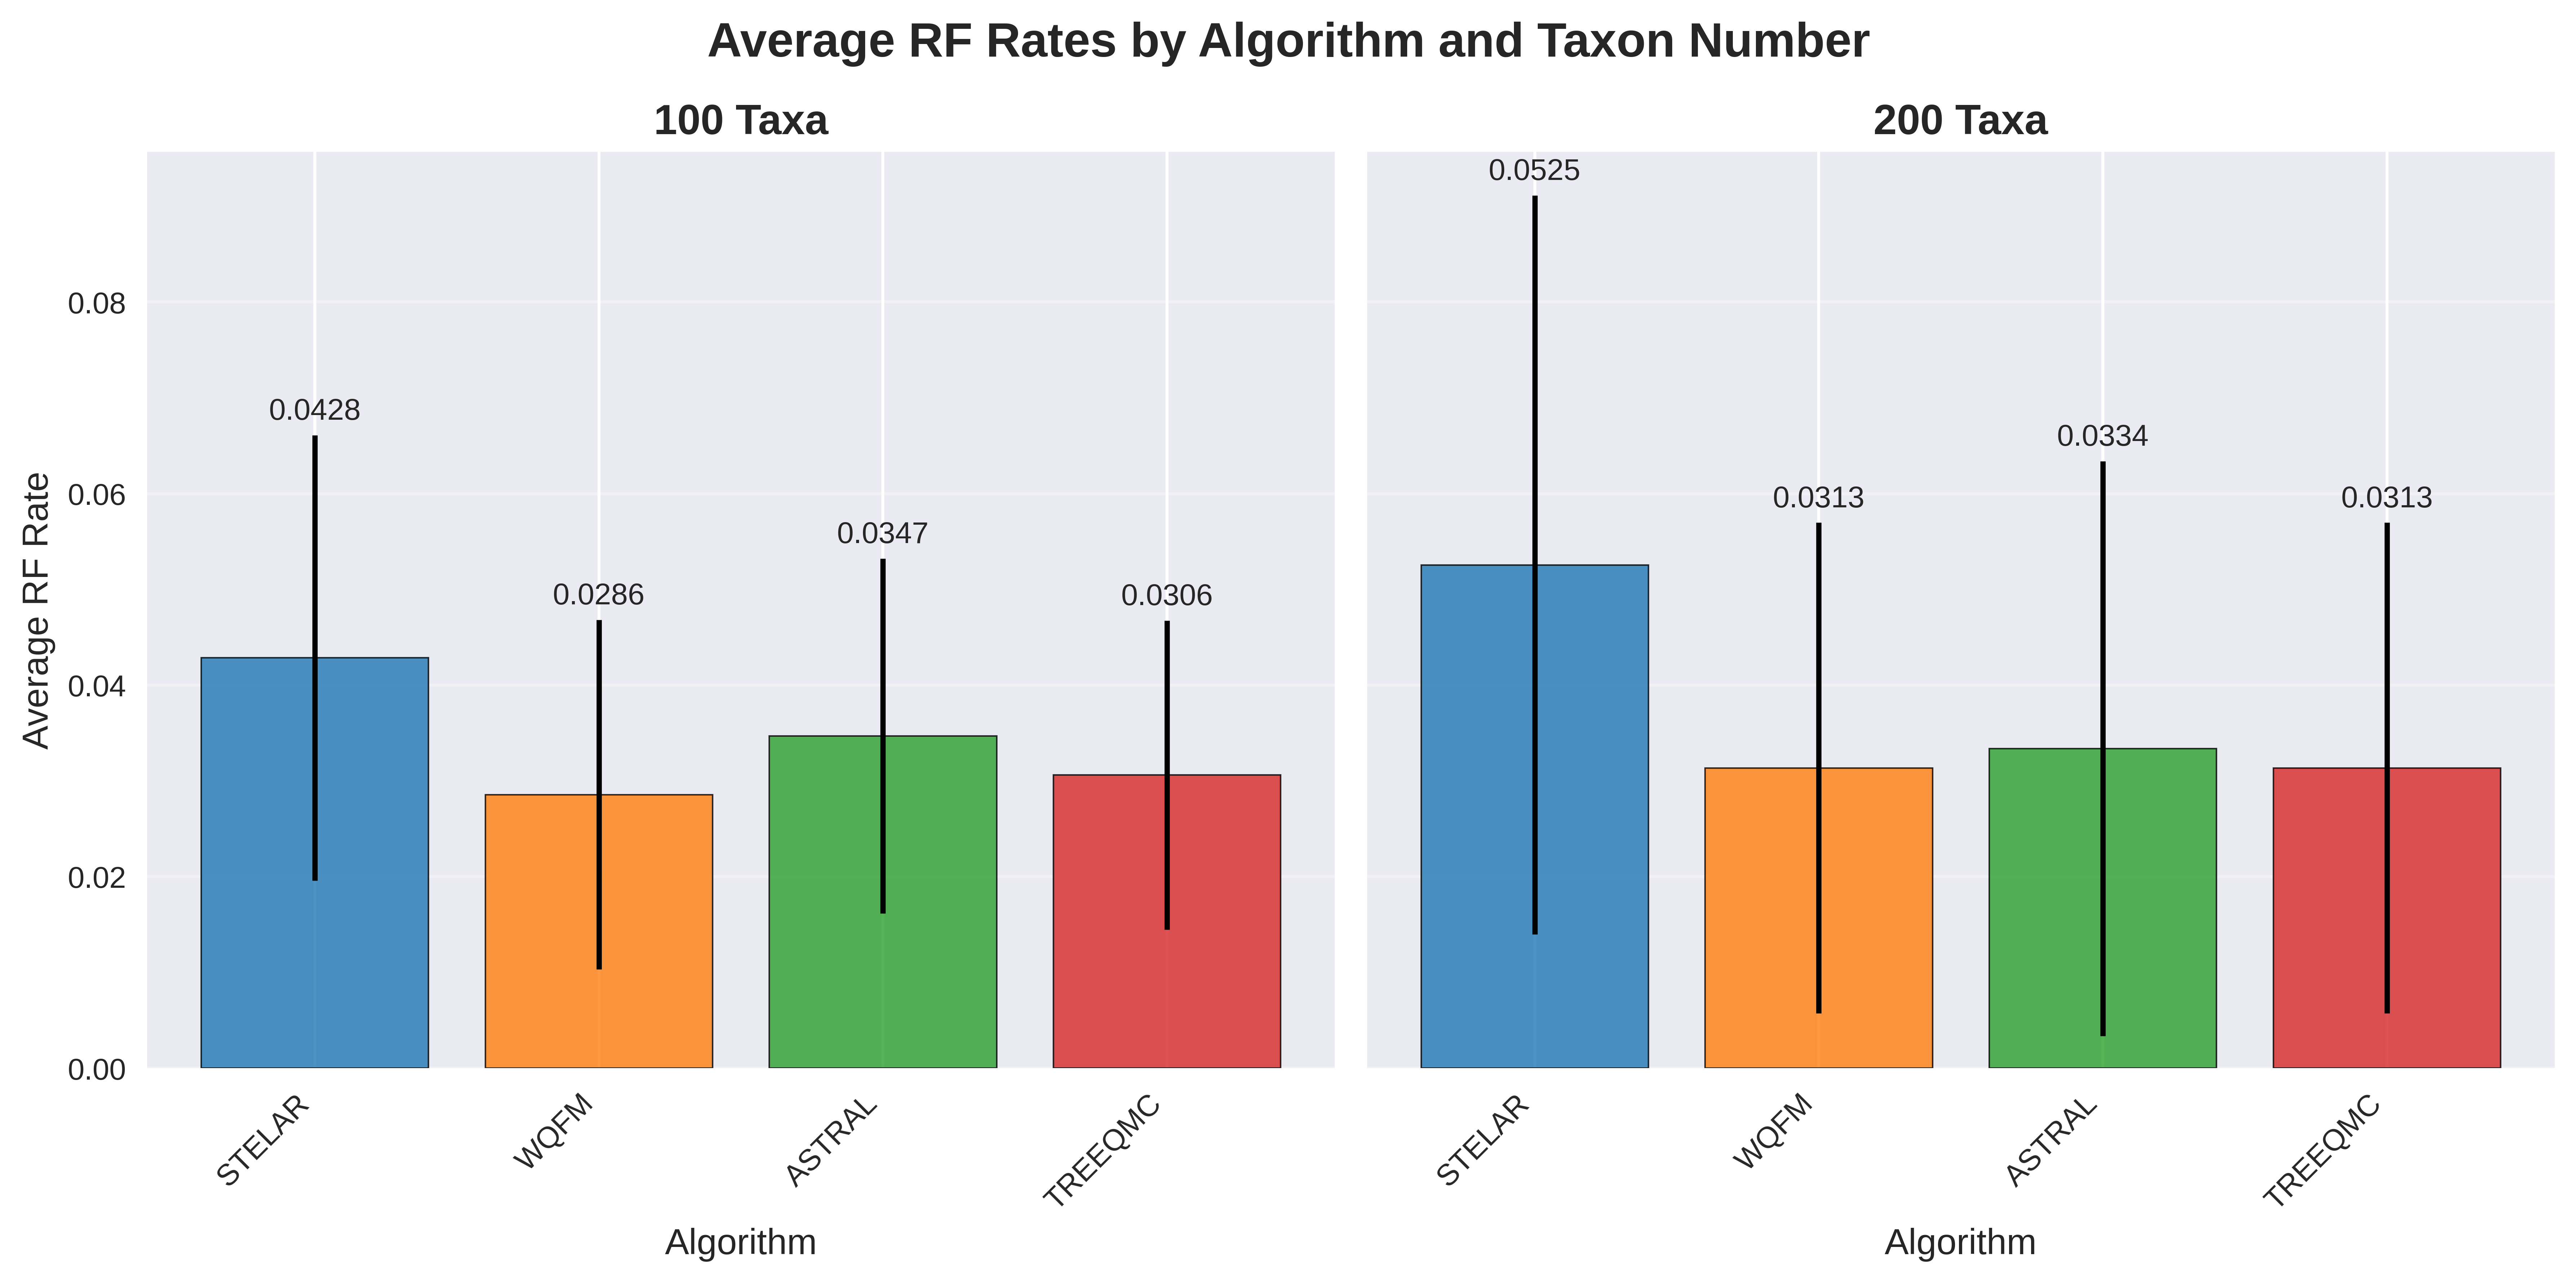
\includegraphics[width=0.8\linewidth]{fig-stx/results/rf_rates_comparison.png}
    \caption{Caption}
    \label{fig:placeholder}
\end{figure}


% \begin{figure}
%     \centering
%     
\includegraphics[width=\linewidth]{fig-stx/results/stelar-scale-taxa.png}
%     \caption{Caption}
%     \label{fig:placeholder}
% \end{figure}

% \begin{table}[h]
% \caption{Running time and memory usage of STELAR with varying number of taxa}
% \centering
% \begin{tabular}{l l l l l}
% \toprule
% No. of Taxa & No. of Gene Trees & Running Time (s) & CPU RAM (MB) & GPU VRAM (MB) \\
% \midrule
% 10000  & 1000 & 87.321   & 11047.477 & 497.664 \\
% 25000  & 1000 & 1176.499   & 18659.977 & 638.976 \\
% 50000  & 1000 & 6660.976   & 54229.543 & 858.544 \\
% 75000  & 1000 & 16901.294   & 77415.117 & 1098.364 \\
% 100000  & 1000 & 30776.740   & 86336.082 & 1330.442 \\
% \bottomrule
% \end{tabular}
% \end{table}

% \begin{figure}
%     \centering
%     
\includegraphics[width=\linewidth]{fig-stx/results/stelar-scale-gt-1k.png}
%     \caption{Caption}
%     \label{fig:placeholder}
% \end{figure}

% \begin{table}[h]
% \caption{Running time and memory usage of STELAR with varying number of gene trees}
% \centering
% \begin{tabular}{l l l l l}
% \toprule
% No. of Taxa & No. of Gene Trees & Running Time (s) & CPU RAM (MB) & GPU VRAM (MB) \\
% \midrule
% 10000  & 1000 & 87.321   & 11047.477 & 497.664 \\
% 10000  & 2500 & 419.918   & 19518.605 & 624.640 \\
% 10000  & 5000 & 1291.352   & 24002.172 & 829.440 \\
% 10000  & 7500 & 2211.381   & 53890.949 & 1008.446 \\
% 10000  & 10000 & 3111.629   & 75593.758 & 1208.248 \\
% \bottomrule
% \end{tabular}
% \end{table}





% \begin{figure}
%     \centering
%     
\includegraphics[width=\linewidth]{fig-stx/results/vary-ils-performance.png}
%     \caption{Caption}
%     \label{fig:placeholder}
% \end{figure}


% \begin{table}[h]
% \caption{Running time of STELAR-X under different ILS conditions}
% \centering
% \setlength{\tabcolsep}{8pt}
% \begin{tabular}{l l c c c c}
% \toprule
% \multicolumn{2}{c}{} & \multicolumn{4}{c}{\textbf{Running Time (s)}} \\
% \cmidrule(lr){3-6}
% No. of Taxa & No. of Gene Trees & ILS-L1 & ILS-L2 & ILS-L3 & ILS-L4 \\
% \midrule
% 10000 & 1000 & 68.12 & 87.32 & 121.61 & 182.68 \\
% 15000 & 1000 & 147.25 & 200.62 & 294.76 & 443.33 \\
% 20000 & 1000 & 339.71 & 563.79 & 999.84 & 1715.54 \\
% 25000 & 1000 & 647.36 & 1176.50 & 2142.89 & 3733.87 \\
% \bottomrule
% \end{tabular}
% \end{table}

% \begin{table}[h]
% \caption{CPU RAM usage of STELAR-X under different ILS conditions}
% \centering
% \setlength{\tabcolsep}{8pt}
% \begin{tabular}{l l c c c c}
% \toprule
% \multicolumn{2}{c}{} & \multicolumn{4}{c}{\textbf{CPU RAM (MB)}} \\
% \cmidrule(lr){3-6}
% No. of Taxa & No. of Gene Trees & ILS-L1 & ILS-L2 & ILS-L3 & ILS-L4 \\
% \midrule
% 10000 & 1000 & 12123.14 & 11047.48 & 11538.92 & 12451.77 \\
% 15000 & 1000 & 16030.71 & 16413.78 & 16454.35 & 16542.80 \\
% 20000 & 1000 & 17530.17 & 18945.68 & 19319.74 & 18463.49 \\
% 25000 & 1000 & 17452.03 & 18659.98 & 19913.23 & 20318.38 \\
% \bottomrule
% \end{tabular}
% \end{table}

% \begin{table}[h]
% \caption{GPU VRAM usage of STELAR-X under different ILS conditions}
% \centering
% \setlength{\tabcolsep}{8pt}
% \begin{tabular}{l l c c c c}
% \toprule
% \multicolumn{2}{c}{} & \multicolumn{4}{c}{\textbf{GPU VRAM (MB)}} \\
% \cmidrule(lr){3-6}
% No. of Taxa & No. of Gene Trees & ILS-L1 & ILS-L2 & ILS-L3 & ILS-L4 \\
% \midrule
% 10000 & 1000 & 491.52 & 497.66 & 501.76 & 514.05 \\
% 15000 & 1000 & 534.53 & 538.62 & 550.91 & 565.25 \\
% 20000 & 1000 & 579.58 & 591.87 & 606.21 & 628.74 \\
% 25000 & 1000 & 624.64 & 638.98 & 659.46 & 681.98 \\
% \bottomrule
% \end{tabular}
% \end{table}



\begin{figure}
    \centering
    
\includegraphics[width=0.9\linewidth]{fig-stx/trees/avian-stelar-circ-normal.png}
    \caption{Caption}
    \label{fig:placeholder}
\end{figure}



\section{Discussion}

\textcolor{blue}{TODO}


\section{Conclusion}

\textcolor{blue}{TODO}


\subsection{Datasets}

\subsubsection{Simulated Datasets}

\begin{enumerate}
    \item 100-taxon, 200-taxon -> accuracy comparison among STELAR , ASTRAL, WQFM-TREE, TREE-QMC

    \item Large Simulated Datasets -> accuracy, runtime, CPU RAM, GPU VRAM

    

    
\end{enumerate}

\subsubsection{Empirical Datasets}

\begin{enumerate}
    \item 1kp plant Dataset - accuracy and runtime
\end{enumerate}

\subsection{Simulation Parameters}

\begin{table}[h!]
\centering

\begin{tabular}{|l|l|}
\hline
\textbf{Parameter Name} & \textbf{parameter Value} \\ \hline
\textbf{Speciation rate} & 0.0000001 \\ \hline
Extinsion rate & 0 \\ \hline
Number of Taxa & 100 \\ \hline
Ingroup divergence to the ingroup ratio & 1.0 \\ \hline
Generations & LogN(1.470055e+01,2.500000e-01) \\ \hline
\textbf{Haploid effective population size} & 400000 \\ \hline
Global substitution rate & LogN(-1.727461e+01,6.931472e-01) \\ \hline
Lineage specific rate gamma shape & LogN(1.500000e+00,1) \\ \hline
Gene family specific rate gamma shape & LogN(1.551533e+00,6.931472e-01) \\ \hline
Gene tree branch specific rate gamma shape & LogN(1.500000e+00,1) \\ \hline
Seed & 22 \\ \hline
% Sequence Length & 1600 \\ \hline
% Sequence base frequencies & Dirichlet(A=36,C=26,G=28,T=32) \\ \hline
% Sequence transition rates & Dirichlet(TC=16,TA=3,TG=5,CA=5,CG=6,AG=15) \\ \hline
\end{tabular}
\vspace{6pt}
\caption{Simulation parameters used for the generation of gene trees and species trees in Simphy}
\label{tab:simphy-params}

\end{table}


\bibliographystyle{unsrt}
% \bibliography{References}
\bibliographystyle{IEEEtran}
\bibliography{references.bib} % NEED TO CHANGE to references.bib

\end{document}

\usepackage{xr}
\usepackage{longtable}
%\externaldocument{main}
\usepackage{subfiles} 
\usepackage{xcolor}
\newcommand{\add}[1]{{\color{black} #1}}
\newcommand{\addb}[1]{{\color{red} #1}}
\usepackage[linesnumbered,ruled,vlined]{algorithm2e}

%\usepackage{booktabs, caption, makecell}
%\renewcommand\theadfont{\bfseries}
% \usepackage{algcompatible}

\renewcommand{\thefigure}{S\arabic{figure}}
\renewcommand{\thetable}{S\arabic{table}}

% \usepackage{algorithmicx}

\usepackage{setspace} % 24 July

\makesavenoteenv{tabular}
\makesavenoteenv{table}

\hypersetup{
    urlcolor=blue,
}


% for moving the page number to left or right

\usepackage{fancyhdr}
\fancyhf{} % clear all header and footers
\renewcommand{\headrulewidth}{0pt} % remove the header rule
\fancyfoot[LE,RO]{\thepage} % Left side on Even pages; Right side on Odd pages
\pagestyle{fancy}
\fancypagestyle{plain}{%
  \fancyhf{}%
  \renewcommand{\headrulewidth}{0pt}%
  \fancyhf[lef,rof]{\thepage}%
}
% end of page numbering related task


\providecommand{\keywords}[1]{\textbf{\textit{Keywords:}} #1}

\providecommand{\runningtitle}[1]{\textbf{\textit{Running title:}} #1}

%Self-Attention Augmented Inception-Inside-Inception Network Improves Protein Secondary Structure Prediction
\title{Supplementary Material to\\title
\author[1,*]{\author[1,*]{Author list}}
}

%\affil[1]{Department of Computer Science and Engineering\\Bangladesh University of Engineering and Technology
%}

%\affil[*]{Corresponding author}
\affil[1]{Department of Computer Science and Engineering\protect\\
Bangladesh University of Engineering and Technology
\protect\\ Dhaka-1205, Bangladesh
}
\affil[$\dag$]{These authors contributed equally to this work}
\affil[*]{Corresponding author: shams\_bayzid@cse.buet.ac.bd, rimpi@cse.buet.ac.bd}
\date{}

%\date{July 2019}

%SAINT: Self Attention Augmented Inception Inside Inception Network Improves Protein Secondary Structure Prediction



\begin{document}

\maketitle

%\runningtitle{SAINT: Accurate and interpretable secondary structure prediction.}\\

%\runningtitle{SAINT: A secondary structure prediction tool.}\\


%\keywords{Protein secondary structure, deep learning, self-attention.}


%\newpage
\pagestyle{plain}
	\tableofcontents

\clearpage
\section{Overview}

These supplementary materials present additional details about the datasets analyzed in this study (Sec. 2), results on simulated and real biological datasets (Sec. 3), running time information (Sec. 6), and also additional tables and figures (Secs. 5 and 7). We also present a comparison between QFM and wQFM, showing the positive impact of including weights in estimating trees by amalgamating quartets (Sec. 4).

\subsection{15-taxa}

\begin{figure}[H]
    
    \includegraphics[width=\linewidth]{15_Taxon_Dataset/plot_QRF_All.pdf}
    \caption{Average Robinson-Foulds distance of ASTRAL-complete, WQFM-complete, WQMC-complete, ASTRAL-incomplete, WQFM-incomplete, WQMC-incomplete, WQFM-imputed, and WQMC-imputed on the \textbf{15-taxon} dataset with different taxa removal rate. We varied the taxa removal from ($6-13\%$) to ($33-40\%$). We analyzed the estimated gene trees only. We show the average RF distance with standard error bars over 10 replicates.}
    \label{fig:RF_WQFM_15_Taxon}
    \end{figure}



% \begin{figure}[H]
%     \centering % <-- added
%     \includegraphics[width=\linewidth]{15_Taxon_Dataset/plot_QM_Species_Match.pdf}
%     \caption{Quartets distribution matching between the true species tree quartet and the dominant complete, incomplete and imputed gene trees quartet distribution. They are computed against different taxa removal rate. The imputed quartet distribution match with the true species tree quartets almost perfectly at higher removal rate.}
%     \label{fig:Quartet Species Match}
%     \end{figure}

% \begin{figure}[H]
%     \centering % <-- added
%     \includegraphics[width=\linewidth]{15_Taxon_Dataset/plot_QM_Species_Mismatch.pdf}
%     \caption{Quartets distribution mismatch between the true species tree quartet and the dominant complete, incomplete and imputed gene trees quartet distribution using different taxa removal rate.}
%     \label{fig:Quartet Species Mismatch}
%     \end{figure}

% \begin{figure}[H]
%     \centering % <-- added
%     \includegraphics[width=\linewidth]{15_Taxon_Dataset/plot_QM_Genes_Match.pdf}
%     \caption{Average quartets distribution matching between the true gene trees quartets and complete, incomplete and imputed quartet distributions.}
%     \label{fig:Quartet Genes Match}
%     \end{figure}


\begin{figure}[H]
    \centering
    \includegraphics[width=\linewidth]{15_Taxon_Dataset/plot_BRC_15_Taxon.pdf}
    \caption{The Bray-Curtis Distance between the quartet distributions of true gene trees and the complete, incomplete and the imputed gene trees for four taxa removal rate  i.e. 1-2, 2-3, 4-5 and 5-6 taxa respectively.}
    \label{fig:BRC_15_taxon}
\end{figure}

\begin{figure}[H]
    \centering
    \includegraphics[width=\linewidth]{15_Taxon_Dataset/plot_JAC_15_Taxon.pdf}
    \caption{The Jaccard Distance between the quartet distributions of true gene trees and the complete, incomplete and the imputed gene trees for four taxa removal rate  i.e. 1-2, 2-3, 4-5 and 5-6 taxa respectively.}
    \label{fig:JAC_15_taxon}
\end{figure}





\subsection{37-taxa}

\begin{figure}[H]
    \centering
    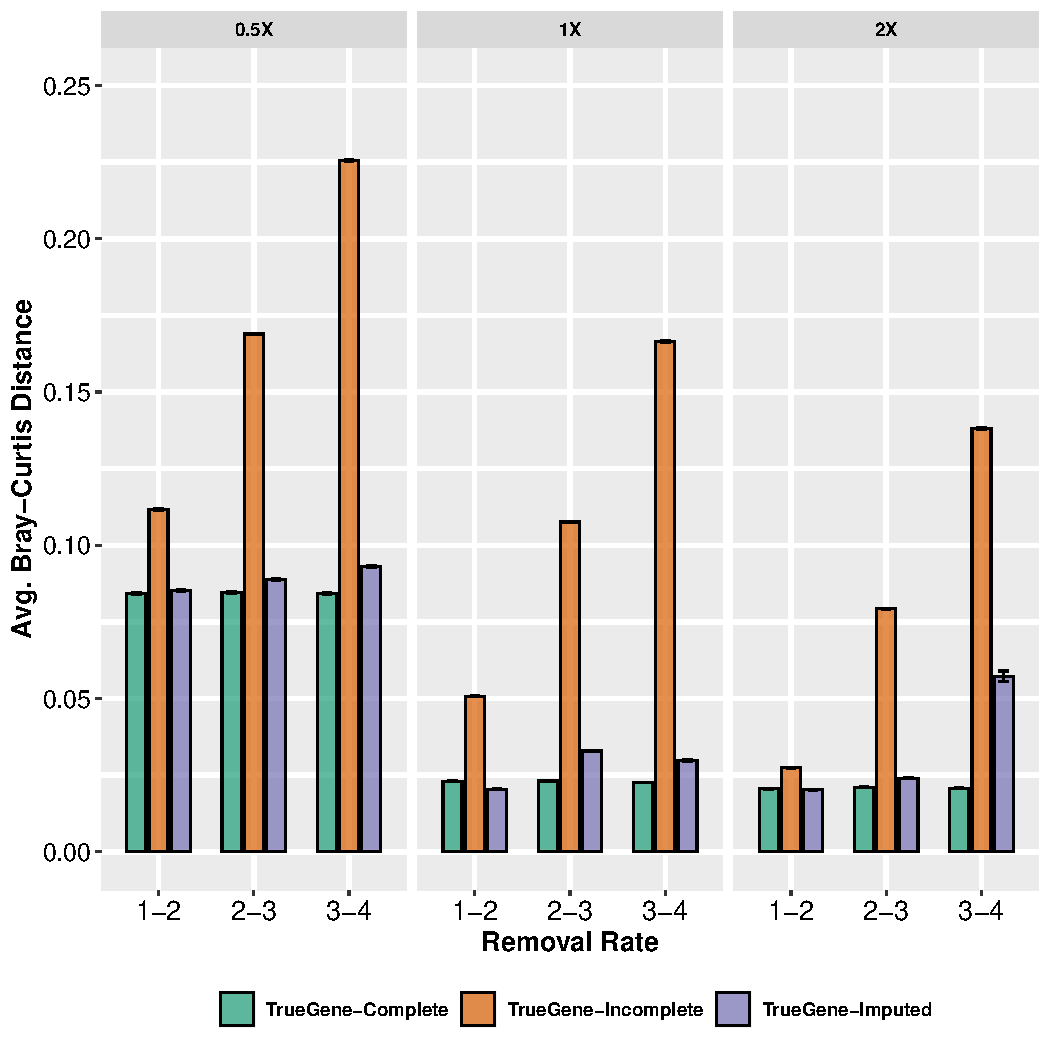
\includegraphics[width=\linewidth]{37_Taxon_Dataset/plot_BRC.pdf}
    \caption{The Bray-Curtis Distance between the quartet distributions of true gene trees and the complete, incomplete and the imputed gene trees for three taxa removal rate  i.e. 1-2, 2-3 and 3-4 taxa respectively.}
    \label{fig:BRC_37_taxon}
\end{figure}

\begin{figure}[H]
    \centering
    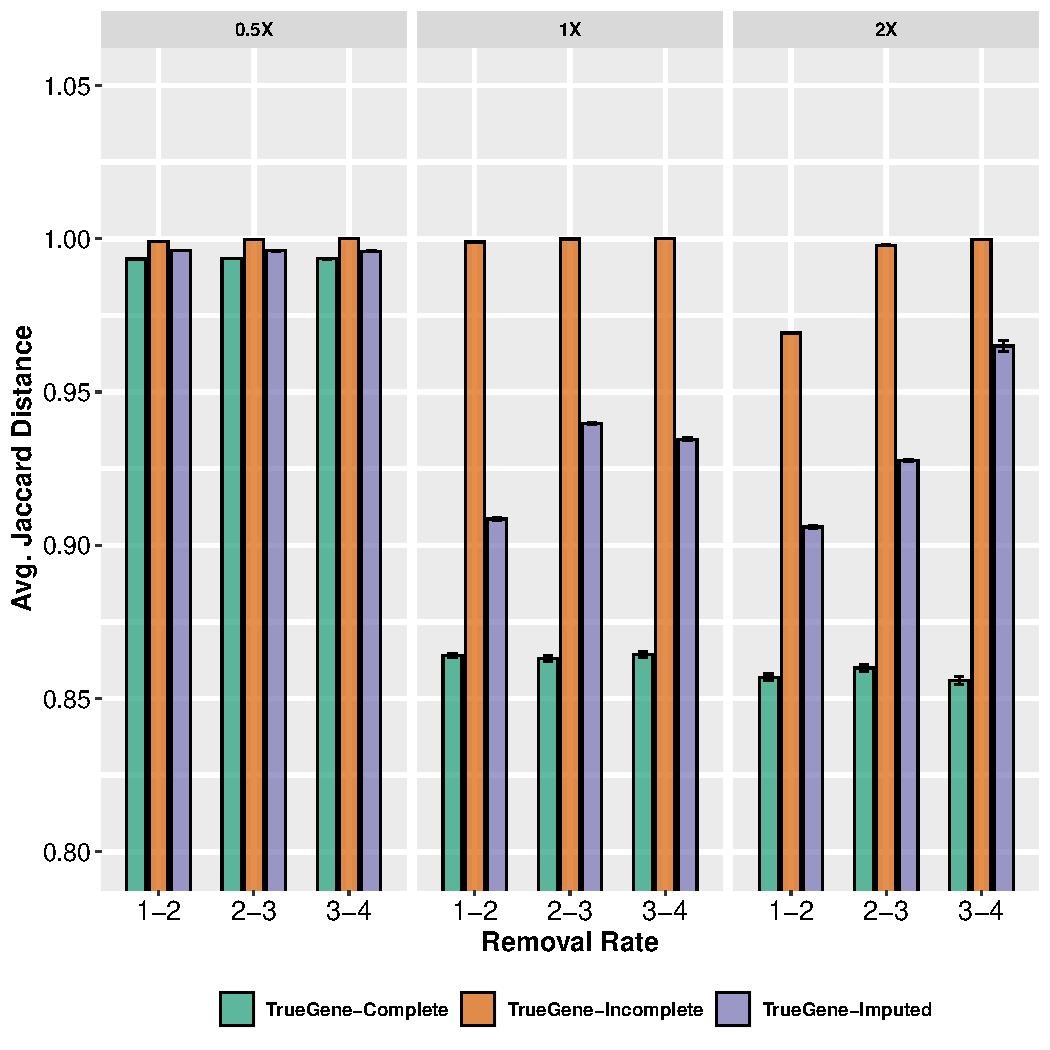
\includegraphics[width=\linewidth]{37_Taxon_Dataset/plot_JAC.pdf}
    \caption{The Jaccard Distance between the quartet distributions of true gene trees and the complete, incomplete and the imputed gene trees for three taxa removal rate  i.e. 1-2, 2-3 and 3-4 taxa respectively.}
    \label{fig:JAC_37_taxon}
\end{figure}

\begin{figure}[H]
    
    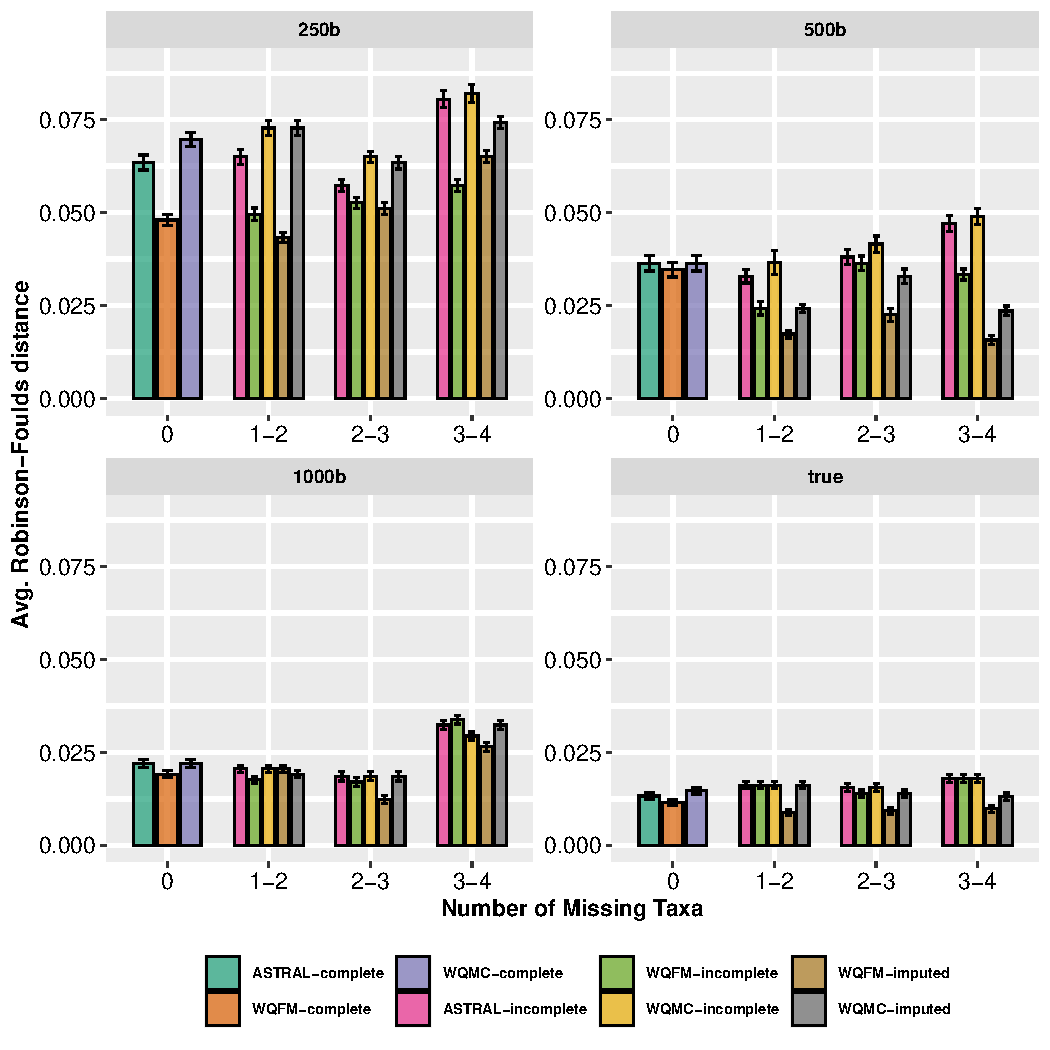
\includegraphics[width=\linewidth]{37_Taxon_Dataset/SequenceLength/plot_QRF_All.pdf}
    \caption{Average Robinson-Foulds distance of Complete(ASTRAL), Complete(WQMC), 
    Incomplete(Astral), Incomplete(WQMC) and Imputed(WQMC) on the \textbf{37-taxon} dataset with different taxa removal rate. We varied the taxa removal from ($6-13\%$) to ($33-40\%$). We analyzed the estimated gene trees only. We show the average RF distance with standard error bars over 20 replicates.}
    \label{fig:RF_Rates_37_Taxon_seqLength_All}
\end{figure}


\bibliographystyle{unsrt}
\bibliography{references.bib}

\end{document}

